\minitoc

\vfill

The goal of this introduction is to acquaint the reader with concepts that are manipulated in this study.
In section~\ref{sec::introduction::urban_3d_reconstruction}, we illustrate what is meant by urban \index{urban!\gls{acr::3d}!model}\gls{acr::3d} models, and specifically, \index{building!model} building \gls{acr::3d} models.
The role of this chapter is also to motivate the need for a semantic \index{building!model!evaluation}evaluation of such models.
Indeed, in section~\ref{sec::introduction::building_model_evaluation}, we address different aspects of building \index{urban!\gls{acr::3d}!model}\gls{acr::3d} model inspection and the issues it raises.
We conclude by stating our contributions (cf. section~\ref{sec::introduction::contributions}) and announcing the structure of the thesis (cf. section~\ref{sec::introduction::structure_of_thesis}).

\clearpage

\section{Urban \gls*{acr::3d} reconstruction}
    \label{sec::introduction::urban_3d_reconstruction}
    \index{\gls{acr::3d}!reconstruction}\gls{acr::3d} reconstruction is a wide research field that interests \index{photogrammetry}Photogrammetry, \index{computer vision}Computer Vision and \index{computer graphics}Computer Graphics communities.
    In summary, the main idea is, using some input sensor data (\gls{acr::lidar} point clouds or stereo images), to acquire the \gls{acr::3d} surface that bounds an object fo interest.
    In \index{\gls{acr::gis}}\gls{acr::gis}, \gls{acr::3d} data is instrumental to model the Earth surface at different scales.
    In particular, the field takes a special focus in \index{urban!area}urban areas.
    Objects present in such scenes obey usually some specific rules that constrain their shape.
    In this section, we dicuss applications of \index{urban!\gls{acr::3d}!model}urban \gls{acr::3d} models (cf. subsection~\ref{subsec::introduction::urban_3d_reconstruction::applications}).
    We tackle, afterwards, the field \index{building!\gls{acr::3d}!model} building \gls{acr::3d} modeling and the issues it raises(cf. subsection~\ref{subsec::introduction::urban_3d_reconstruction::building_3d_modeling}).
    This section ends, in subsection ~\ref{subsec::introduction::urban_3d_reconstruction::challenges}, with a listing of some important technical challenges that are still to be overcome in this domain.

    \subsection{Applications of urban \gls*{acr::3d} models}
        \label{subsec::introduction::urban_3d_reconstruction::applications}
        In what follows, we present a brief survey of \index{urban!model!application} urban \gls{acr::3d} models applications.
        A more comprehensive study was presented in~\textcite{ijgi4042842}.
        The goal is to persuade the reader of the relevance of urban \index{urban!\gls{acr::3d}!model}\gls{acr::3d} modeling and how much concerned can everybody can be.
        Indeed, urban \gls{acr::3d} models answer various needs: scientific, societal, environemental and adminidtrative.

        \subsubsection{Administration related challenges}
            Administrative bodies need to document land usage in an effort to efficiently manage territories.
            Cadastre is a tool that helps track ownership and usage of a each land parcel.
            Cadastral records are produced and maintained to define fiscal policies.
            Cadastral data, since conception, was presented in the form of \index{\gls{acr::2d}!maps}\gls{acr::2d} maps~\parencite{billen20033d}.
            Although many urban planning norms were always formulated taking into account height, or depth, information \parencite{brasebin20183d}, the need for a \index{\gls{acr::3d}!cadastre}\gls{acr::3d} cadastral management was made relevant with the advent of complex architectural features~\textcite{ijgi4042842}.
            To illustrate this case, we show, in figure~\ref{fig::3d_cadastre_need_example}, how \gls{acr::2d} cadastral maps are insufficient when it comes to modeling overhangs.\\
            \begin{figure}
                \centering
                \includegraphics[width=\textwidth]{images/introduction/3d_model_applications/3d_cadastre}
                \caption{\label{fig::3d_cadastre_need_example} Example of a problematic situation where \gls{acr::3d} cadastre would be of help and \gls{acr::2d} maps fail~\parencite{ijgi4042842}.}
            \end{figure}
        \subsubsection{Urban planning related challenges}
            Urbanization raises some serious issues that need to be adressed.
            Consequently, decision makers, and all stakeholders in general, need to have at their disposal adequate tools.
            \index{\gls{acr::3d}!model}\gls{acr::3d} models are, in this sense, suitable as shown hereafter.\\
            While the previously presented \index{\gls{acr::3d}!cadastre}\gls{acr::3d} cadastre describes an urban scene at a certain time, urban plannars need the access to the same kind of information but in the future also.
            In fact, they need to know in advance the impact of urban norms they write on the evolution of their zone of interest. 
            One of the issues they study is \index{urban sprawl}urban sprawl~\parencite{ludlow2006urban}.
            The goal is to limit, as far as possible, \index{land occupation}land occupation~\parencite{TANNIER2012128} and predict the shape of the urban scene~\parencite{brasebin20183d} by tuning local urban plans.
            This can be acheived, for instance, through simulation, at different scales, based on a formal description of urban planning norms as shown by the work of~\textcite{Colomb17a}.
            In reality, the \gls{acr::2d} city footprint is not sufficient to assess its capacity to contain people.
            One has to compute the number of habitable units, which depends on the height of buildings.
            This motivates the need of \gls{acr::3d} data as shown in Figure~\ref{fig::3d_simulation}.
            The \index{vizualization} vizualization and \index{simulation}simulation of urban zones can be equally helpfull for \index{public consultation}public consultation~\parencite{WU2010291}.\\
            \begin{figure}[htpb]
                \centering
                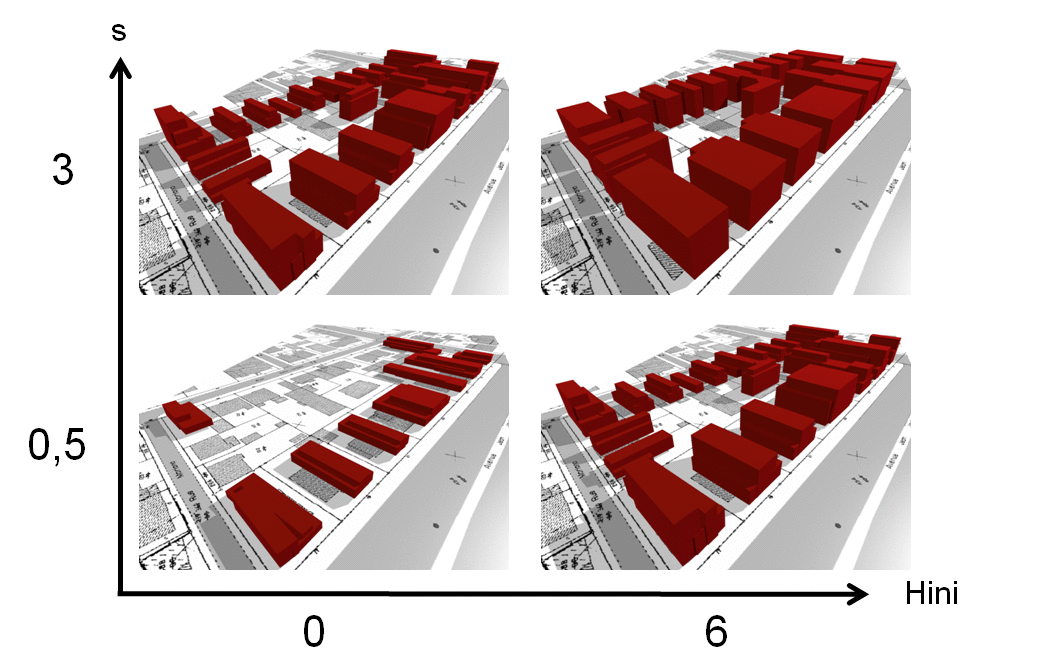
\includegraphics[width=\textwidth]{images/introduction/3d_model_applications/simplu}
                \caption{
                    \label{fig::3d_simulation} Example of \gls{acr::3d} urban scene simulated based on known urban norms with different values of parameters using the SimPLU3D tool developped by~\textcite{brasebin2017stochastic}.
                    Urban planners can assess the projected urban density of future districts for better decision making.
                }
            \end{figure}
            \begin{figure}[htpb]
                \centering
                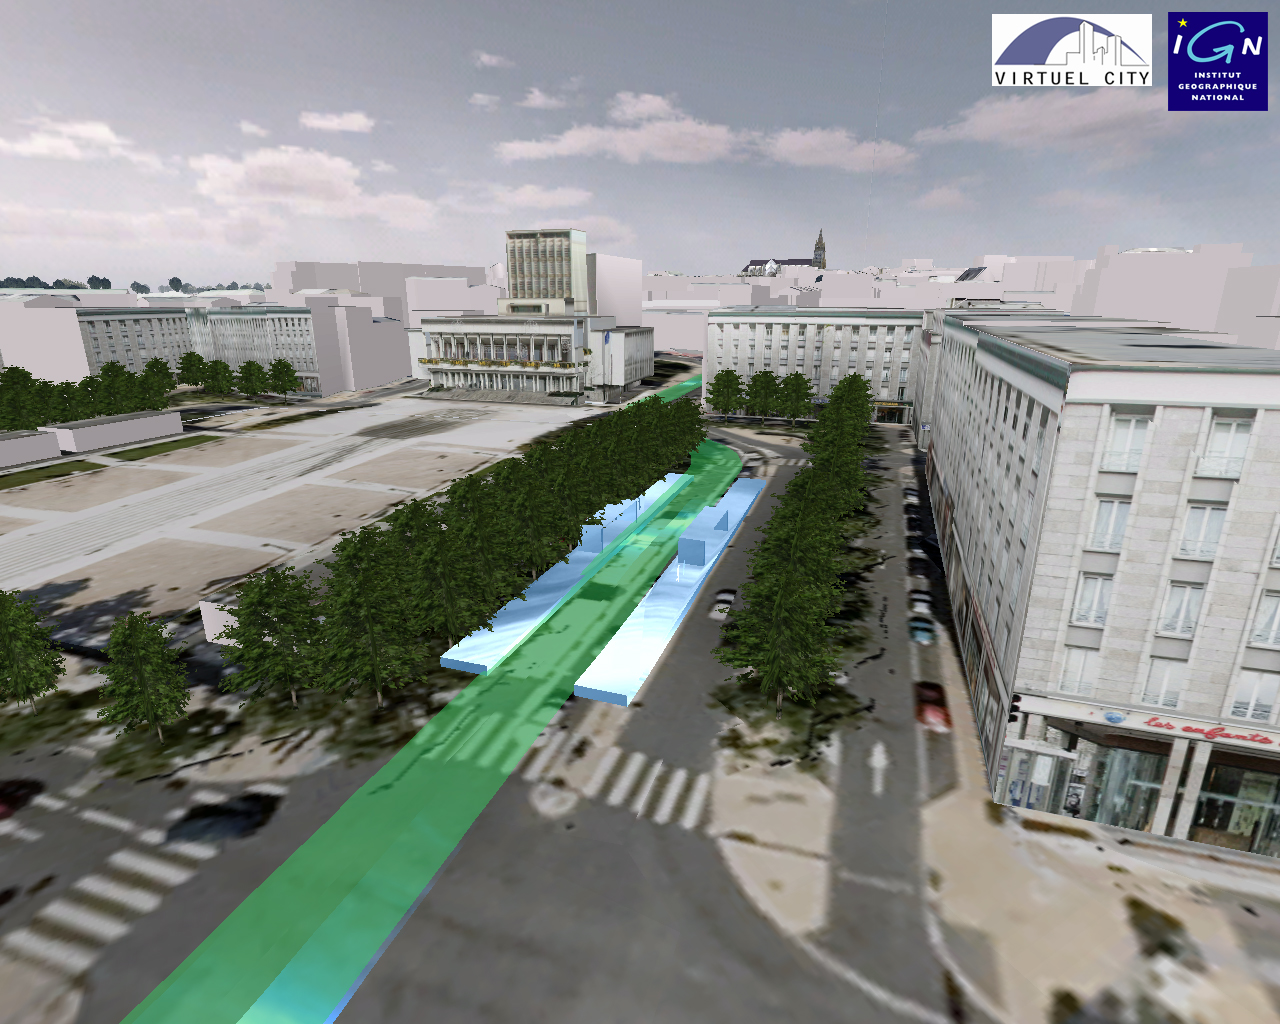
\includegraphics[width=\textwidth]{images/introduction/3d_model_applications/brest_tramway}
                \caption{
                    \label{fig::public_consultation} Example of the use of city \gls{acr::3d} models in public consultation.
                    This image was produced using the \gls{acr::ign} Bati3D\textsuperscript{\textregistered} models of Brest, France.
                    The goal is to simulate the impact of the tramway line to be built on the urban landscape.
                }
            \end{figure}
            Related to urban planning, \gls{acr::3d} models could be used as a reference for other planners.
            It could be used to describe the flow of vehicles and pedestrians in an urban environement as illustrated in~\textcite{vanhoey2017varcity}.
            In addition, it could be used in physical simulations for urban applications.
            For instance, Communication companies need to have a \gls{acr::3d} model of urban scenes to predict \textbf{signal propagation} in the goal of \textbf{optimal network planning}~\parencite{yun2007radio}.
            It can be useful also for \textbf{flood simulation}.
            Predicting the height of overflowing water requires inherently a \gls{acr::3d} information.
            This is the usecase of~\textcite{varduhn2015multi}, where \gls{acr::3d} models are used to assess the flood risk.
            Such information could be instrumental for evacuation planning or for insurance managers.
            In the same direction, one can simulate \textbf{fire propagation}~\parencite{dimitropoulos2010fire} or estimating noise propagation in urban scenes~\parencite{stoter20083d} (\textit{cf.} Figure~\ref{fig::noise_propogation}).
            \begin{figure}[htpb]
                \centering
                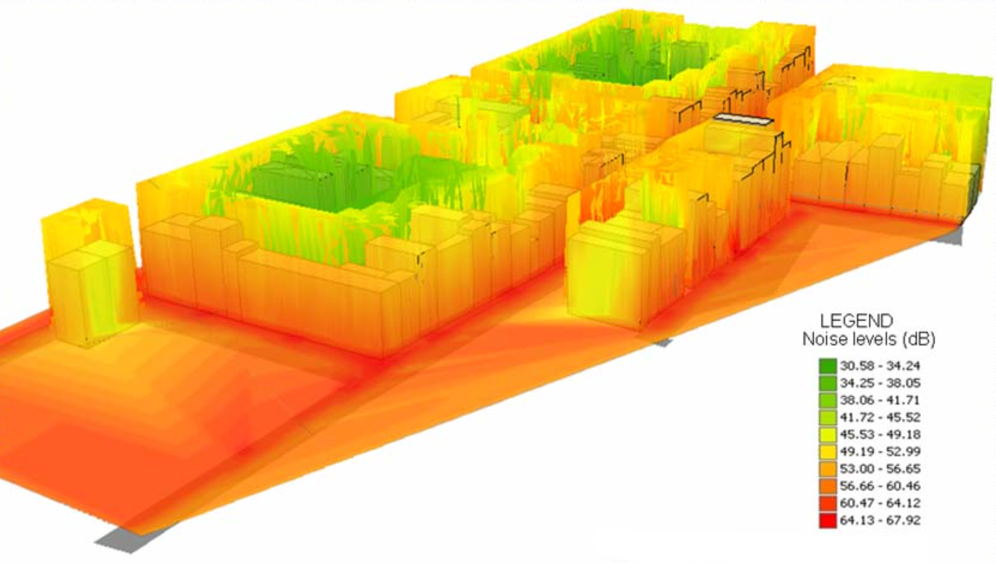
\includegraphics[width=\textwidth]{images/introduction/3d_model_applications/noise_simulation}
                \caption{
                    \label{fig::noise_propogation} Example of \textbf{noise propagation} simulation using \gls{acr::3d} city models~\parencite{kurakula2007gis}.
                }
            \end{figure}
            All these simulation derived informations could be fed to decision makers in order to better plan the cities of tomorrow.

        \subsubsection{Environmental challenges}
            Environement preservation is a all the more important in the forecoming years.
            Urban settlement are one of the most biggest energy consumers.
            A more efficient energy utilization is necessary to sustain the frantic growth of urban areas.
            This motivates the need to quantify the energy consumption of urban settlements~\parencite{WATE20153372} or retrofitting costs~\parencite{previtali2014automatic}.
            ~\textcite{biljecki2015propagation} use also \gls{acr::3d} models of buildings in order to predict solar irradiation.
            In fact, solar potential estimation can be useful for assessing the benefits of expensive solar panels projects.
            This kind of studies can also be applied in urban planning as the simulations could be undergone for future urban developpements.\\
            \begin{figure}[htpb]
                \centering
                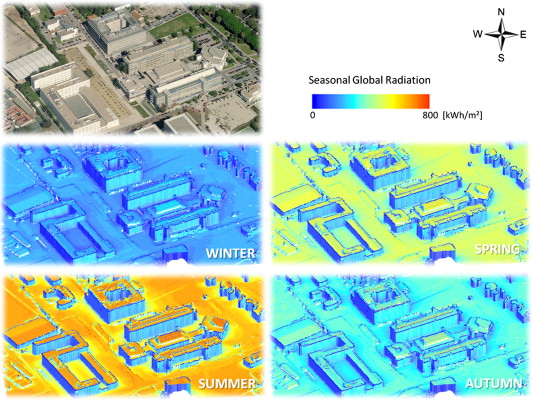
\includegraphics[width=.7\textwidth]{images/introduction/3d_model_applications/solar_potential}
                \caption{
                    \label{fig::solar_potential} Solar potential estimation using building \gls{acr::3d} models~\parencite{redweik2013solar}.
                    The slope, orientation and dimensions of roofs are determinant factors in computing solar irradiation.
                }
            \end{figure}
            Another big environemental issue that affects cities is air pollution.
            Indeed, it has serious implications on human health as demonstrated in~\textcite{pascal2013assessing} and~\textcite{chen2013evidence}.
            In order to understand its dynamics, researchers simulate the local air flow (\textit{i.e.} the city microclimate) using computational fluid dynamics.
            This requires a detailed knowledge of the scenes layout.
            One way to acquire this information is through \index{urban!\gls{acr::3d}!model}\gls{acr::3d} models of urban settlements~\parencite{ujang2013unified}.
       
        \subsubsection{Autonomous navigation related challenges}
            Autonomous navigation has seen a great technological leap in recent years.
            Localization is an important step in visual navigation~\parencite{bonin2008visual}.
            \Gls{acr::3d} models play an important role in visual localization~\parencite{piasco2018survey, ijgi4042842}.\\
            The basic idea is to match an image with a (textured or not) known \gls{acr::3d} model of the city~\parencite{arth2015instant, ardeshir2014gis, cham2010estimating, christie2016semantics} as shown in Figure~\ref{fig::navigation}.
            \begin{figure}[htpb]
                \begin{subfigure}{.18\textwidth}
                    \begin{center}
                        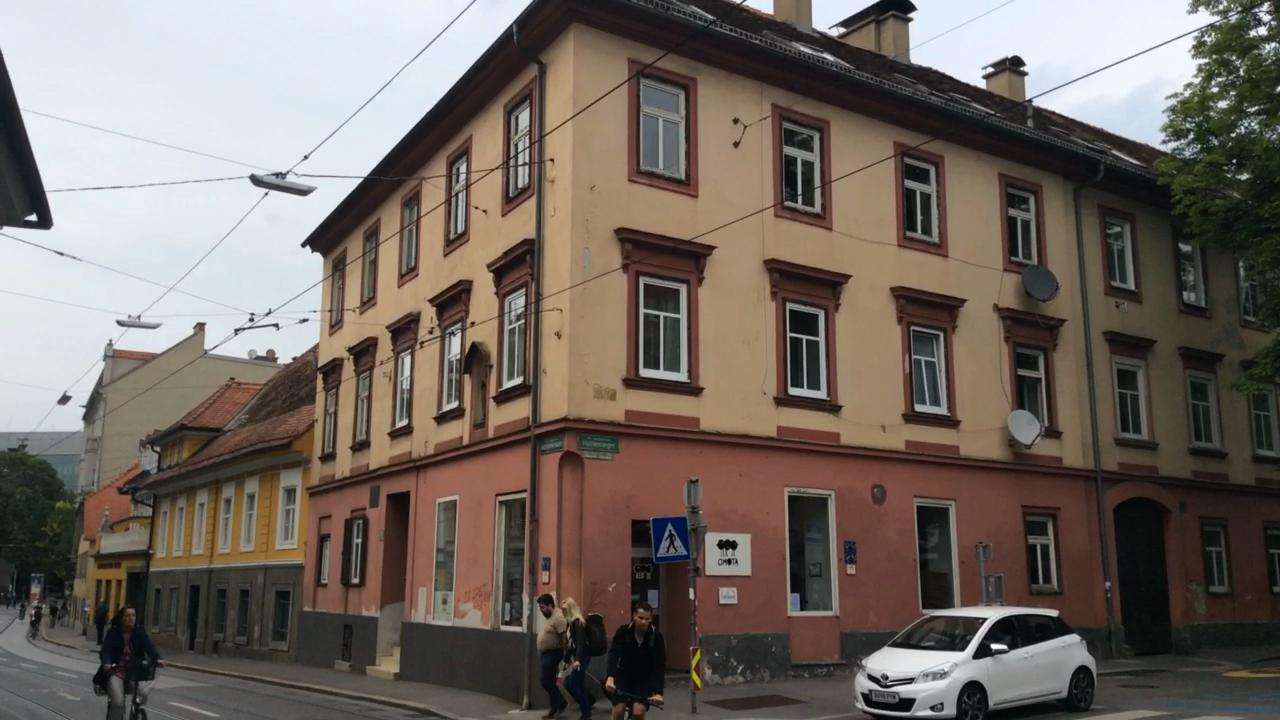
\includegraphics[width=\textwidth]{images/introduction/3d_model_applications/pose_estimation/input_image}
                        \caption{\label{subfig::input_image} Input image}
                    \end{center}
                \end{subfigure}
                \hfill
                \begin{subfigure}{.18\textwidth}
                    \begin{center}
                        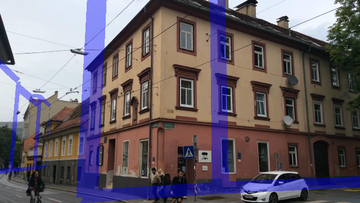
\includegraphics[width=\textwidth]{images/introduction/3d_model_applications/pose_estimation/init_pose}
                        \caption{\label{subfig::init_pose} Initial estimation}
                    \end{center}
                \end{subfigure}
                \hfill
                \begin{subfigure}{.18\textwidth}
                    \begin{center}
                        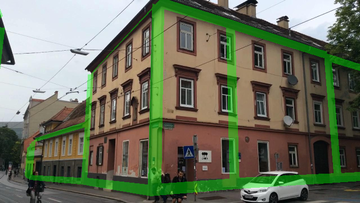
\includegraphics[width=\textwidth]{images/introduction/3d_model_applications/pose_estimation/best_pose}
                        \caption{\label{subfig::final_pose} Final estimation}
                    \end{center}
                \end{subfigure}
                \hfill
                \begin{subfigure}{.18\textwidth}
                    \begin{center}
                        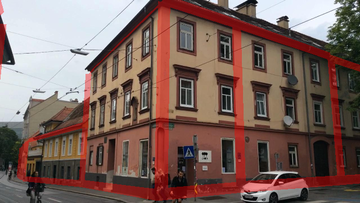
\includegraphics[width=\textwidth]{images/introduction/3d_model_applications/pose_estimation/ground_truth}
                        \caption{\label{subfig::gt_pose} Ground truth}
                    \end{center}
                \end{subfigure}
                \hfill
                \begin{subfigure}{.18\textwidth}
                    \begin{center}
                        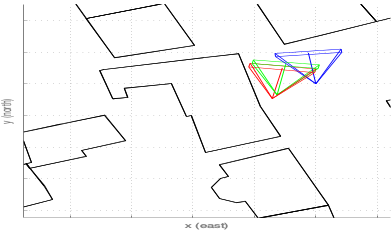
\includegraphics[width=\textwidth]{images/introduction/3d_model_applications/pose_estimation/pose_viz}
                        \caption{\label{subfig::viz} Different poses.}
                    \end{center}
                \end{subfigure}
                \caption{
                    \label{fig::navigation} Position estimation that relies on urban \gls{acr::2d5} models.
                    The initial pose is derived from a sensor measurement that is not reliable.
                    In Subfigures~\ref{subfig::init_pose}(\textit{resp.}~\ref{subfig::final_pose} and~\ref{subfig::gt_pose}), the \gls{acr::2d5} model is projected on the image using the initial pose (\textit{resp.} the refined pose and the ground truth one).
                    The \gls{acr::2d5} model helps refine the camera pose~\parencite{armagan2017semantic}.
                    It is shown in the last graph(\textit{cf.} Subfigure~\ref{subfig::viz}), where the final estimation (green) is closer to the ground truth (red) than the initial one (blue)~\parencite{armagan2017semantic}.
                }
            \end{figure}
            Once the image matched, one can retrieve an absolute 6-\gls{acr::dog} pose estimation.
            This is especially helpfull in urban canyons as shown in~\textcite{piasco2018survey}.\\
            This can be applied also for indoor environments, such as social cues aware robots navigating alongside humans~\parencite{gupta2018social} or industrial grade robots\addref.
       
        \subsubsection{Entertainement related challenges}
            \gls{acr::3d} models appeals also to various agents in the entertainement industry.
            One of the first examples that comes to mind is the video games community~\parencite{watson2008procedural}.
            In their seek of reality, in order to engage the most customers as possible, studios reproduce entire cities as a virtual playing ground for the game story.
            We can cite the "Spider-Man" virtual New-York city\footnote{
                \href{https://www.polygon.com/2013/9/25/4702318/under-the-hood-of-infamous-second-son-hyper-real-seattle}{Under the hood of Infamous: Second Son's hyper-real Seattle}
            }\footnote{
                \href{https://www.polygon.com/e3/2018/6/12/17453588/spider-man-ps4-new-york-city-avengers-demo-preview}{How Spider-Man PS4’s New York City compares to the real thing}
            } or the realistic facsimile of Seattle in "Infamous Second Son"\footnote{
                \href{http://www.businessinsider.fr/us/spider-man-ps4-new-york-city-2018-9}{I'm blown away by the virtual New York City of 'Spider-Man' on PlayStation 4 — here's how it compares to the real thing}
            } as instances of such use.\\
            Tourism can also benefit from such models.
            In fact, virtual touring has become more attainable with works like~\textcite{koutsoudis20073d}.
            For instance, tourists can use it to prepare their trip by familiarizing themselves with the city they are visiting.
            This can be possible through mixed or augmented reality as shown by~\textcite{devaux20183d} (\textit{cf.} Figure~\ref{subfig::augemented_reality}).
            It can also be employed in the service of art.
            Actually,~\textcite{aubry2014painting} and~\textcite{russell2011automatic} illustrated how it is possible to align paintings or photographs with \gls{acr::3d} scenes(\textit{cf.} Figure~\ref{subfig::historical_pose}).\\
            \begin{figure}[htpb]
                \begin{subfigure}{.48\textwidth}
                    \begin{center}
                        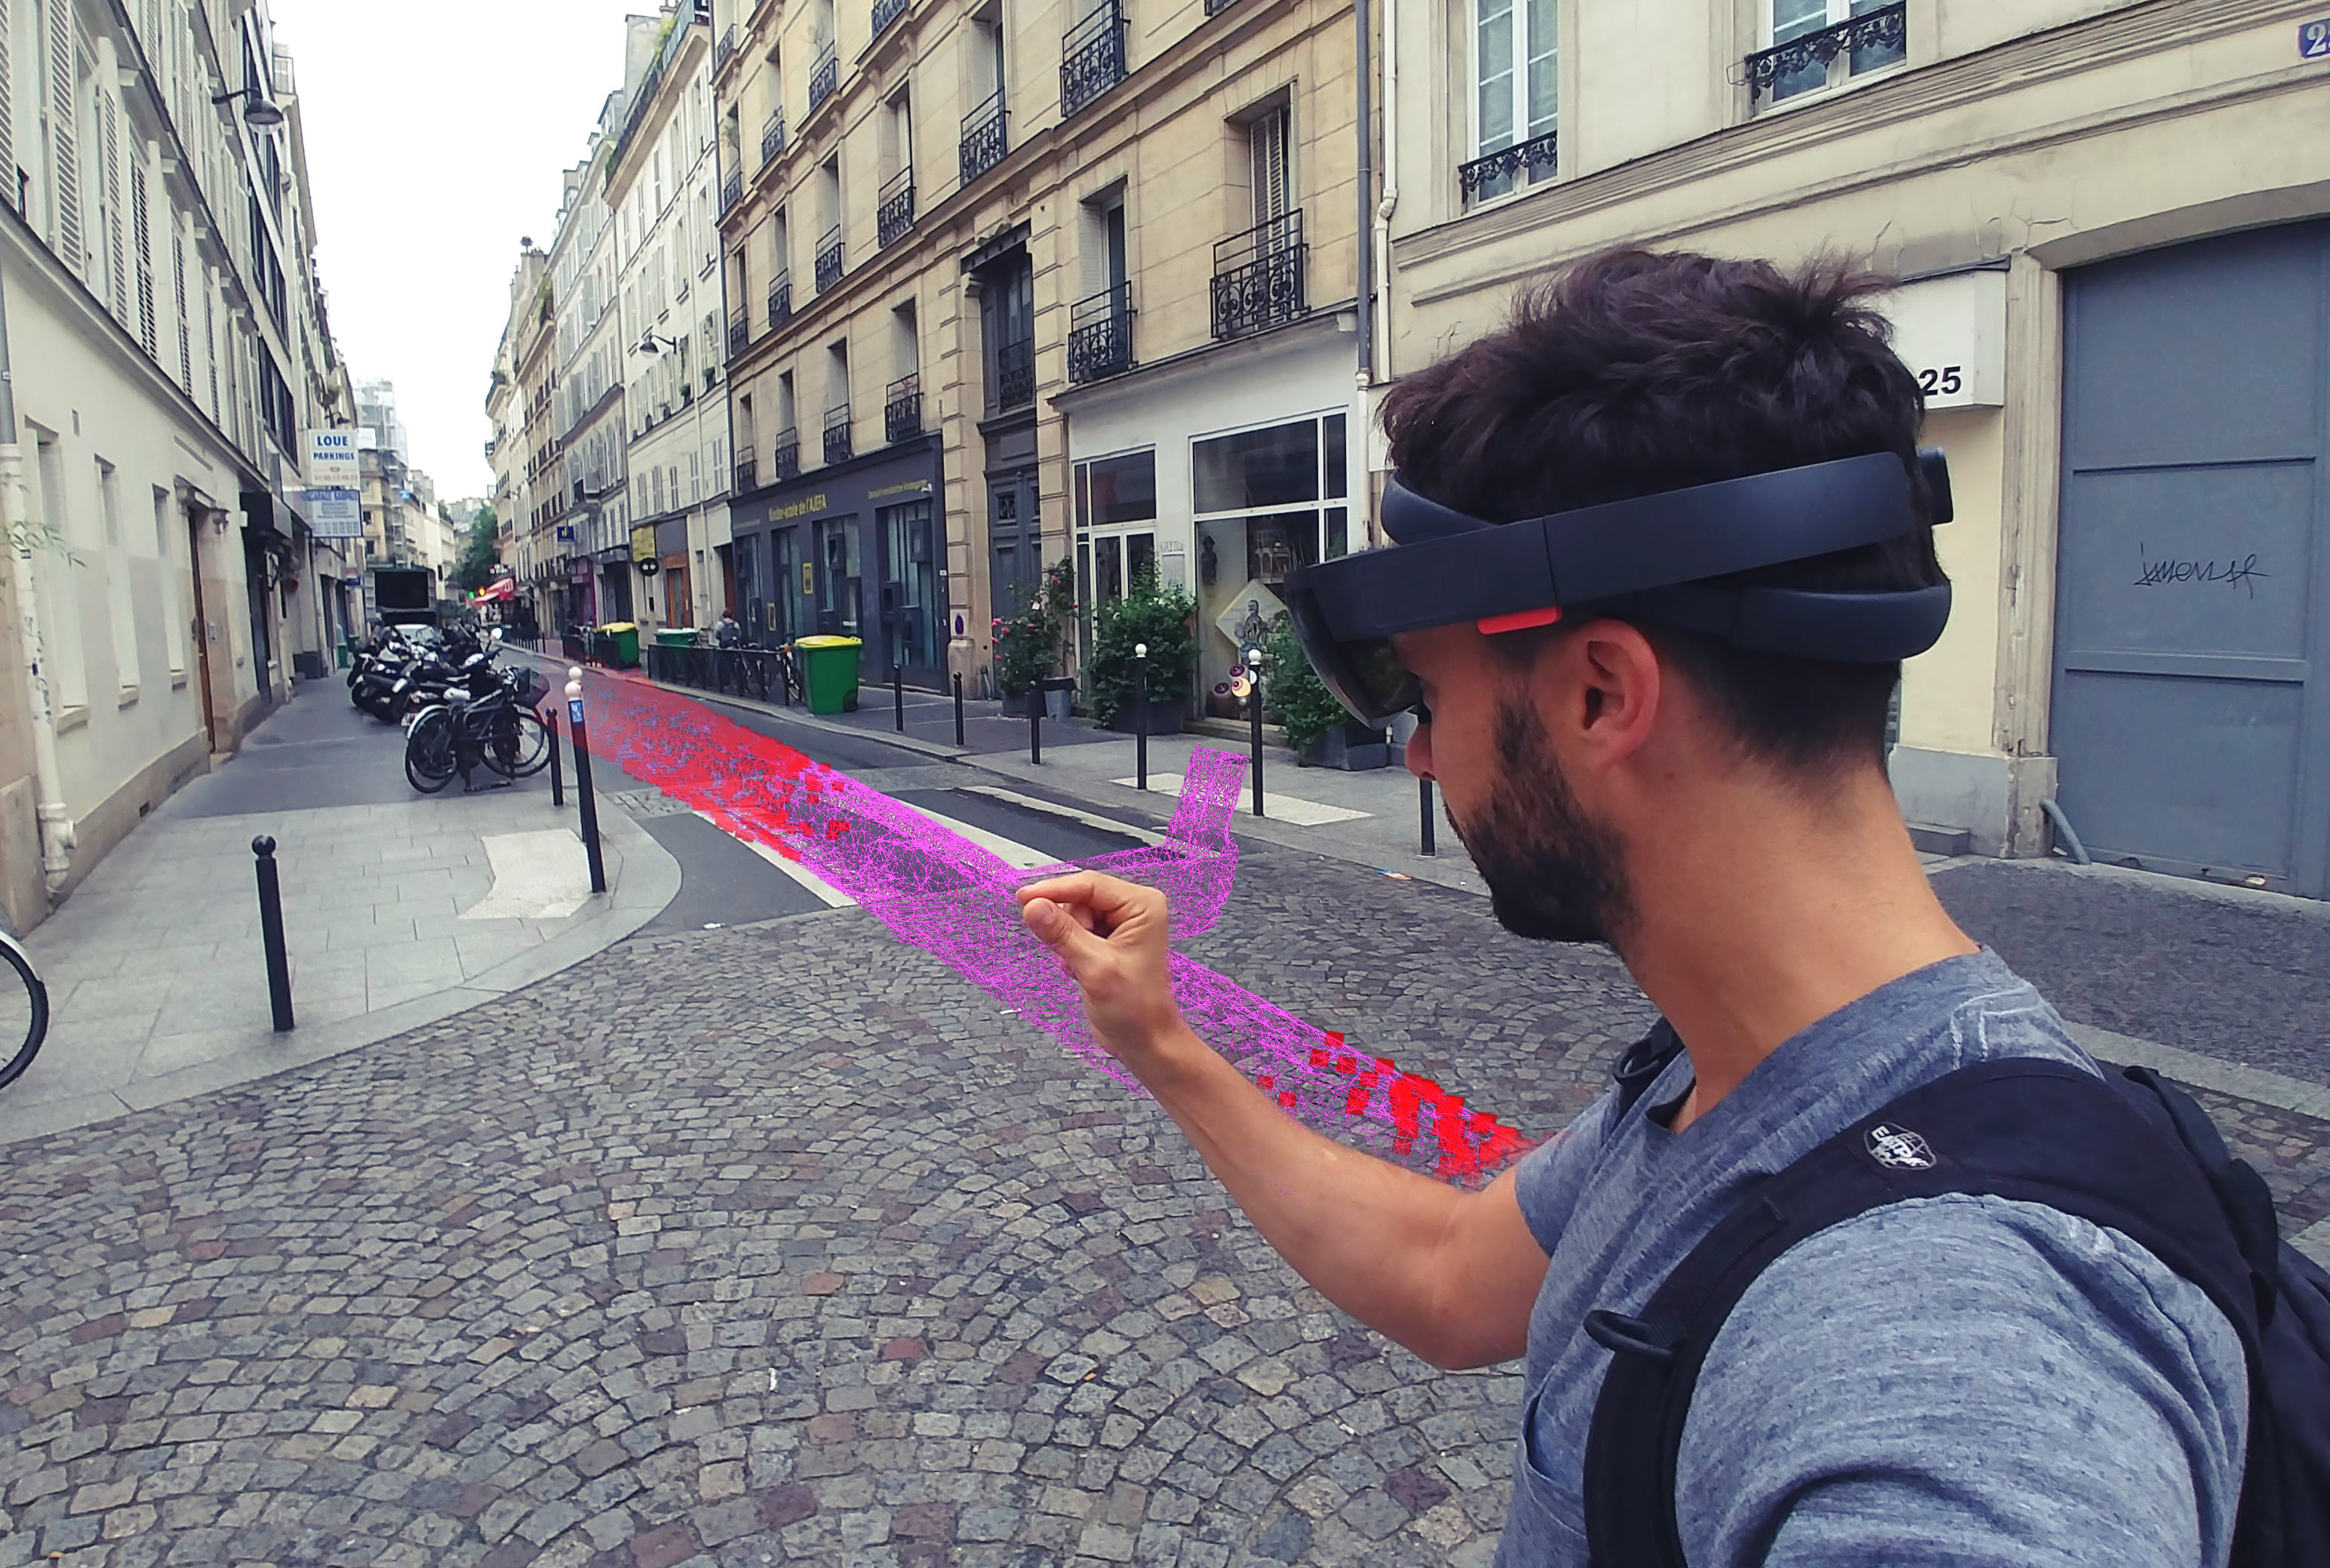
\includegraphics[width=\textwidth]{images/introduction/3d_model_applications/insitu_sewer_hololens}
                        \caption{\label{subfig::augemented_reality} Virtual vizualization of sewers in Paris based on the \gls{acr::3d} model of the city~\parencite{devaux20183d}.}
                    \end{center}
                \end{subfigure}
                \hfill
                \begin{subfigure}{.48\textwidth}
                    \begin{center}
                        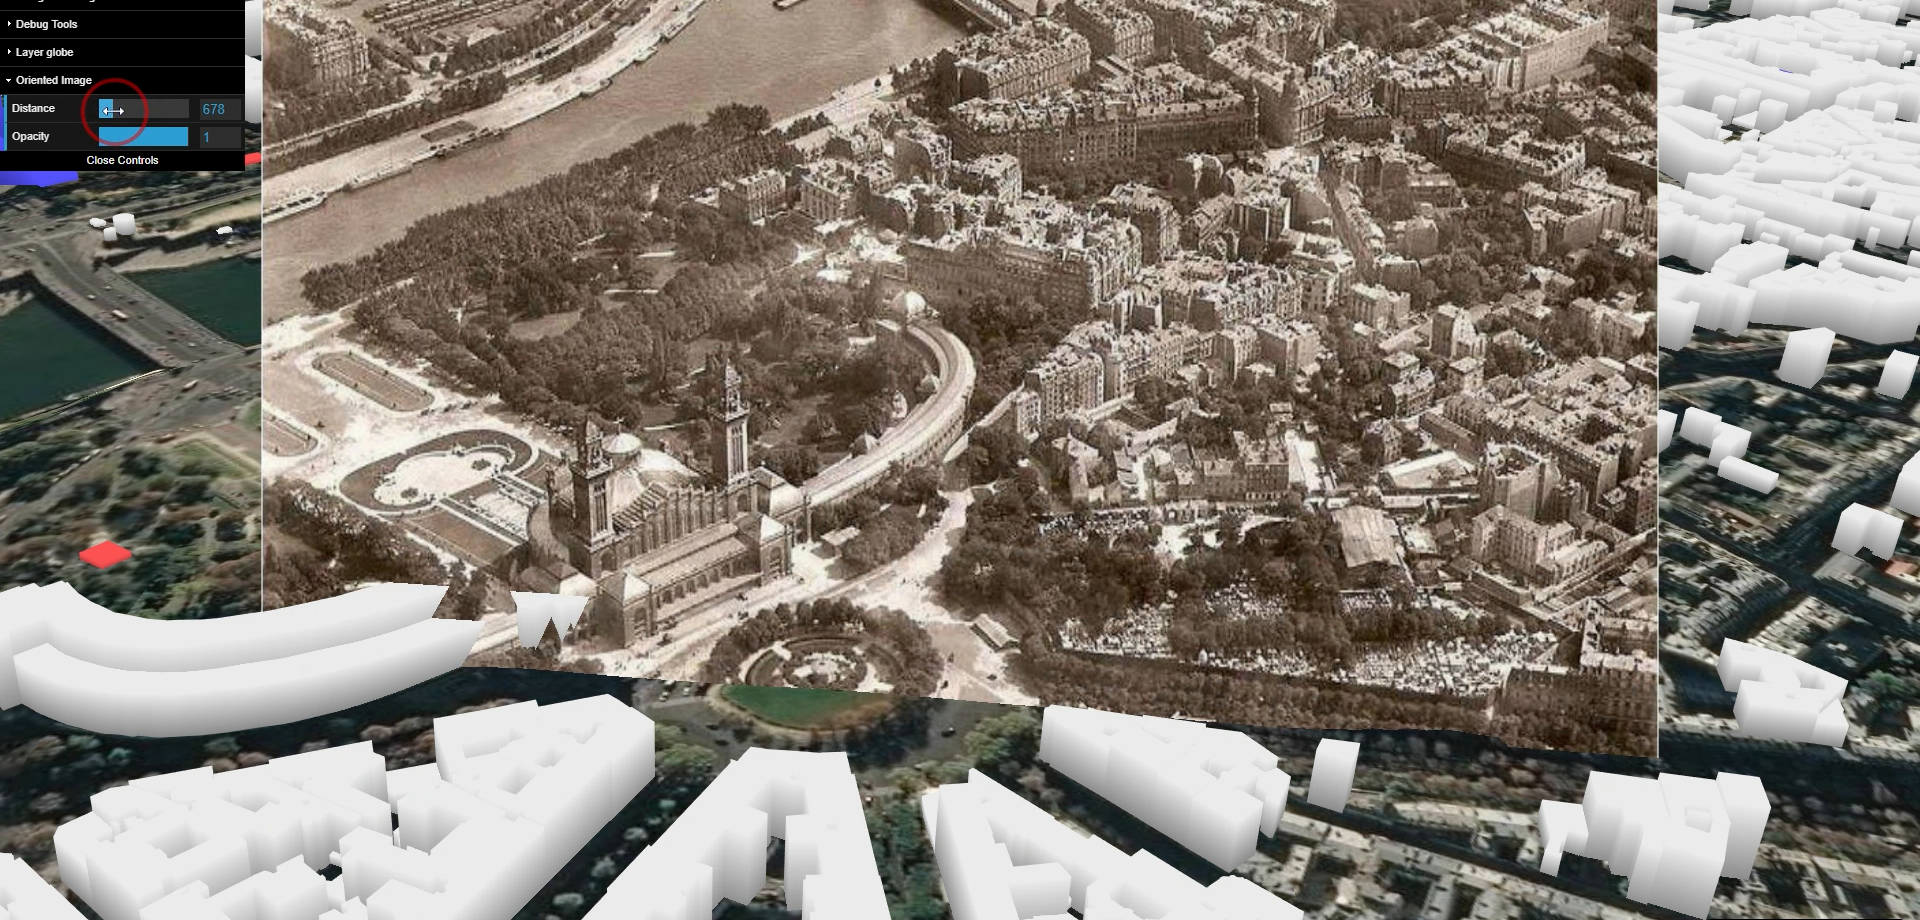
\includegraphics[width=\textwidth]{images/introduction/3d_model_applications/trocadero_historical}
                        \caption[
                            Pose estimation of a historical aerial image of Trocadero square (Paris, France) that was registered~\parencite{harrach2019interactive} to a city \gls{acr::3d} model visualized with iTowns~\parencite{devaux2012web}.
                        ]{
                            \label{subfig::historical_pose} Pose estimation of a historical aerial image of Trocadero square (Paris, France) that was registered~\parencite{harrach2019interactive} to a city \gls{acr::3d} model visualized with iTowns\footnotemark~\parencite{devaux2012web}.
                        }
                    \end{center}
                \end{subfigure}
                \caption[
                    Examples of \gls{acr::3d} model applications in the entertainement field (images are courtesy of Alexandre Devaux)
                ]{
                    \label{fig::entertainement} Examples of \gls{acr::3d} model applications in the entertainement field (images are courtesy of Alexandre Devaux\footnotemark).
                }
            \end{figure}
            This last work could be also used to help marketers sell living units.
            \addtocounter{footnote}{-1}
            \footnotetext{
                \href{http://www.itowns-project.org}{iTowns project}
            }
            \addtocounter{footnote}{1}
            \footnotetext{
                \href{http://recherche.ign.fr/labos/matis/~devaux}{Alexandre Devaux website}
            }
            Indeed, customers can, for example, visit a digitally reconstructed appartement and virtually furnish it~\parencite{kim2019planar}.
            Another application is living unit pricing.
            In fact, one would not have to travel to the asset location in order to assess it.
            Markerters can do so using its \gls{acr::3d} model.
            For instance, one of the determining factors in estimating buildings is the fa\c{c}ade visibility.
            The latter can be simply measured using building models, as shown by~\textcite{albrecht2013assessing}.

        \subsubsection{Security related challenges}
            Security and emergency fields are not the exception when it comes to the utilization of city \gls{acr::3d} models~\parencite{kwan2005emergency, ruppel2011designing}.
            For instance,~\textcite{chen2014application} shows how these models could be used for ladder trucks optimal deployement planning by firefighters.
            It can also be used to determine safe margins in the case of bomb disposal operations.
            This can be possible through explosion simulation in the urban environement of interest~\parencite{willenborg2015simulation}.\\
            \begin{figure}[htpb]
                \centering
                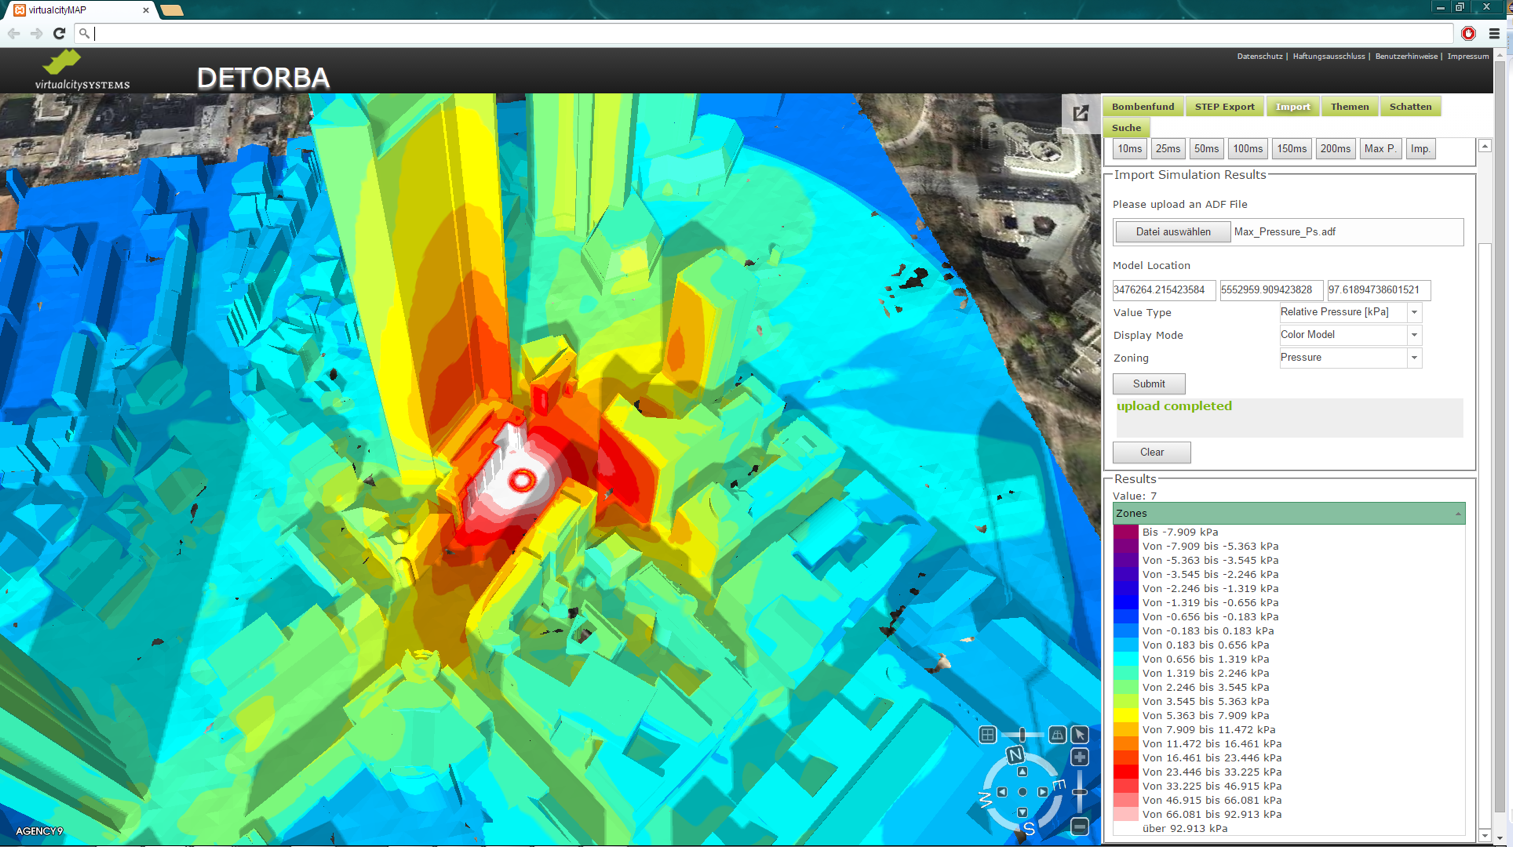
\includegraphics[width=\textwidth]{images/introduction/3d_model_applications/explosion_simulation}            
                \caption{
                    \label{fig::explosion_simulation} Explosion simulation in urban environments.
                }
            \end{figure}
            Security forces can equally benefit from the same models.
            \gls{acr::3d} models can be used to help analysing crime scenes~\parencite{wolff2009towards}.
            It can also be helpfull for crime prevention as proved by~\textcite{wolff2008geospatial}.
            These models could be instrumental in military applications~\textcite{zlatanova2002trends, budroni2010automatic}.
            Military forces could, indeed, use building \gls{acr::3d} model based augmented reality to train for intervention scenarii, such as hostage rescue operations.

    \subsection{Building \gls*{acr::3d} modeling}
        \label{subsec::introduction::urban_3d_reconstruction::building_3d_modeling}
        We have seen, previously, how city \gls{acr::3d} models can be instrumental.
        They have a large range of applications in entertainement, industry, security, urbanization and sustainable developpement.
        In this work, the focus is put on outdoor, rather than indoor, modeling.\\
        Precisely, we will raise, herein, the issue of large scale outdoor city modeling.
        We will see how building reconstruction has a prominent role in the field.
        Afterwhat, we will discuss different building model acquisition techniques and how it influences their quality.
        We end with an examination of semantics in building models.

        \subsubsection{Large scale outdoor city modeling}
            Not all urban items enjoy the same importance.
            This is particularly true when modeling city scapes.
            For this purpose, all different urban elements are analysed based on temporal and spatial dimensions.
            First, urban elements are grouped into different groups depending on how fast they undergo change.
            \gls{acr::3d} modeling is discussed depending on this mentionned categorization.
            Afterwhat, the spatial differentiation would be used to explain how buildings concentrate the most interest in urban \gls{acr::3d} modeling.\\

            Urban environments are temporally dynamic in nature~\parencite{vanhoey2017varcity}.
            However, constituent items do not evolve with uniform speed.
            Therefore, urban objects are distinguished depending on their change rate.
            Pedestrians --- as well as all living animals in general --- and transportation vehicles are in perpetual movement.
            Water bodies and vegetation, in urban scenes, evolve with an annual or seasonal period.
            Last comes city furniture, roads, bridges, buildings and terrain which have a much lower change frequency.
            We proceed, herein, to study how each of these three groups are modeled in \gls{acr::3d}.\\

            Besides technical difficulties, there are ethical and legal issues when reconstructing \gls{acr::3d} models of humans and vehicles.
            Indeed, accurate reconstruction involves person indentification.
            This has proven to be an intricate subject, as proved by~\textcite{tavani2011ethics} and~\textcite{thornton2010individual}.
            Adding to the previous discussion about the high temporal frequency of such objects, seeking the most faithfull models proves to be superfluous.
            In fact, one can populate city models by generic \gls{acr::cad} models of these humans~\parencite{shao2007autonomous} and vehicles.
            Even more so, a lot of aspects of human/vehicle and city interactions do not require \gls{acr::3d} modeling.
            For instance,~\textcite{lovaas1994modeling} can simulate pedestrian traffic flow, which is inherently a \gls{acr::2d} problem\footnote{
                We can safely assume that human do not fly in 2019.
            }, without requiring \gls{acr::3d} human models.\\
            There is little or no work, as far as we know, that is interested in water body \gls{acr::3d} modeling in urban areas.
            Vegetation can be modeled in details using \gls{acr::lidar} acquisition~\parencite{omasa20063d}.
            It is, however, too demanding in ressources and pointless in a large scale context.
            Trees are usually modeled by template matching, such as the ellipsoidal form model in~\textcite{lafarge_ijcv12}, or by generic, species dependent, \gls{acr::cad} models like in~\textcite{iovan2008detection}.\\
            \begin{figure}[htpb]
                \centering
                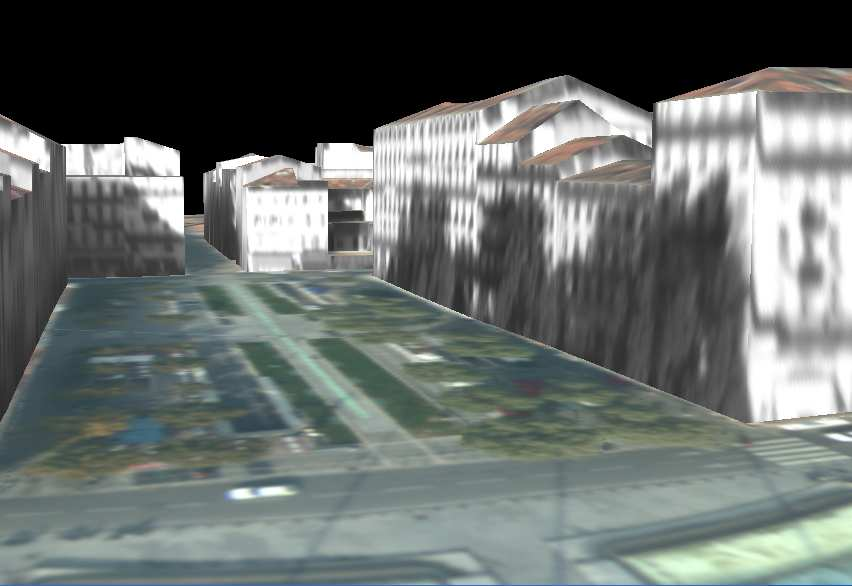
\includegraphics[width=.48\textwidth]{images/introduction/modeling_trees_1}
                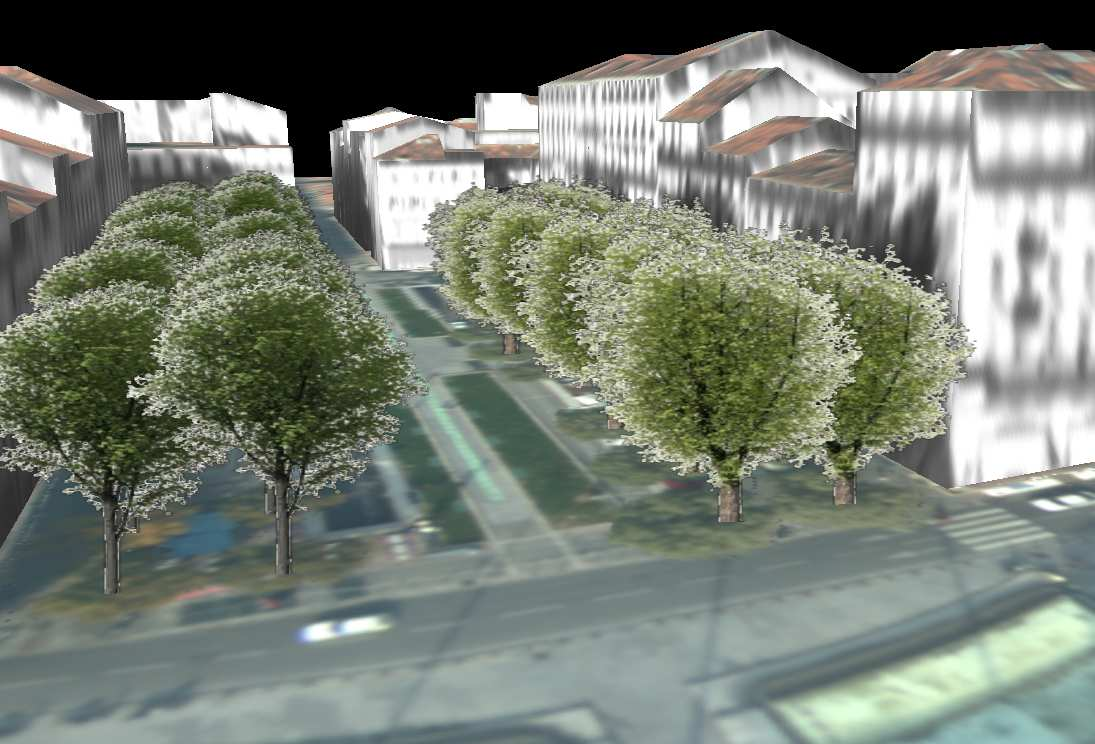
\includegraphics[width=.48\textwidth]{images/introduction/modeling_trees_2}
                \caption{
                    \label{fig::3d_tree_models} The city model is populated with generic models of trees depending on their class~\parencite{iovan2008detection}.
                }
            \end{figure}
            Regarding the first and second groups, was proven, the lack of motivation for precise \gls{acr::3d} reconstruction, in a large scale setting.
            Exhibiting less temporal volatility, precise modeling of items from the third group seems to be easier.
            In fact, terrain relief can be modeled simply from a \gls{acr::dsm} or a \gls{acr::dtm}.
            Although not being so easy to detect~\parencite{mnih2010learning}, roads could be naturally modeled using simple planar structures.
            On the other hand, city furniture, bridges and buildings are more complex.
            While detailed accurate models are needed for buildings and bridges, they are not necessary for city furniture.
            Indeed, it is, for instance, pointless to model each single road sign.
            One would only need to detect its class and reconstruct it, accordingly, using a generic \gls{acr::cad} model portaying the same meaning~\parencite{soheilian2013detection}.\\
            \begin{figure}[htpb]
                \centering
                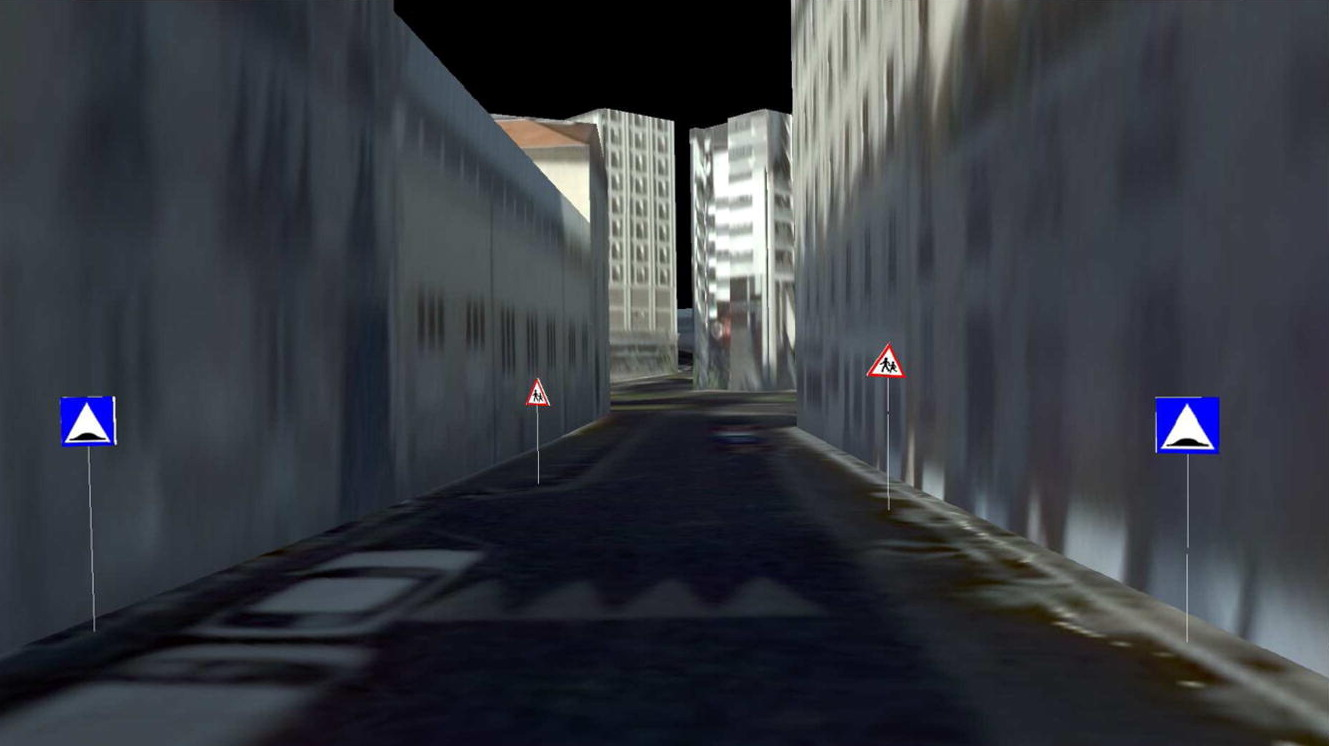
\includegraphics[width=\textwidth]{images/introduction/modeling_road_signs}
                \caption{
                    \label{fig::3d_road_signs_models} The city model is populated with detected road signs using \gls{acr::cad} models~\parencite{soheilian2013detection}.
                }
            \end{figure}

            Based on the previous temporal frequency differentiation analysis, we narrowed down the urban elements that need special consideration in modeling to two: buildings and bridges. 
            Actually, we can rule out the latter owing to, this time, a spatial frequency categorization.
            In terms of land cover, the most occuring objects in an urban environement are roads, vegetation and buildings \addref.
            Hence, modeling these three objects becomes vital in order to obtain a viable urban \gls{acr::3d} model.
            We have seen previously how roads and vegetation could be satisfactorily reconstructed using relatively simple models.
            This is, however, not the case of buildings.
            That is why, out of all urban features, buildings seem to attract the most attention in urban \gls{acr::3d} modeling.

        \subsubsection{Building \gls*{acr::3d} modeling}
            Before discussing further on the different types of building models, a definition is provided.
            A building \gls{acr::3d} model is a cartographic product which represents the surface of the building in question.
            The latter is a generalization of the reality.
            The goal is not to represent all the details meticulously.
            However, the model should not part from the real geometry of the building of interest.
            Thus, geometric fidelity is weighted against generalization.
            The right compromise is chosen based the final user needs.
            This issue will later intervene often in this work.

            Discussed herein are types of building models.
            Scale of reconstruction is a main factor in dividing the latter into two classes (\textit{cf.} Figure~\ref{fig::bim_vs_gis}).
            At a small scale, \gls{acr::bim} or \gls{acr::cad} models are easy to use.
            On the contrary, \gls{acr::gis} models are more suitable at a large scale.\\

            \gls{acr::bim} models are volumetric in nature:
            Each element is represented by a volumetric primitive.
            These models are bottom-up.
            A \gls{acr::bim} model is manually constructed as a blueprints of a building before being constructed.
            It is then supposed to follow the buildings evolution in time until its destruction.
            This is the most detailed possible virtual representation of a building.\\
            However, it does not come without its own issues.
            First, we can see that it rules out all buildings that preceded the technology, especially, historical buildings.
            Secondly, since this type of models require a high interaction with experts, in order to follow the state of the real buildings, it would be almost impossible the fact that the model does not diverge from the reality\addref.
            Last but not least, are the geometric issues, like self-intersections and non 2-manifoldness, that these models display as most \gls{acr::bim} tools do not perform geometric sanity checks.\\

            \begin{figure}[htpb]
                \centering
                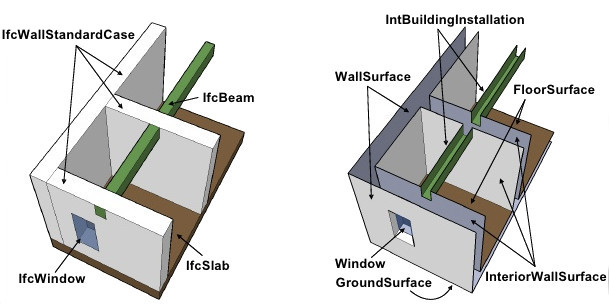
\includegraphics[width=\textwidth]{images/introduction/bim_vs_gis}            
                \caption{
                    \label{fig::bim_vs_gis} \gls{acr::ifc} and CityGML representations of the same object (building storey): \gls{acr::bim} is an inherently volumetric model while \gls{acr::gis} represent the surface of the building~\parencite{nagel2009conceptual}.
                }
            \end{figure}

            In contrast, \gls{acr::gis} models represent rather the surface of buildings.
            The goal is to describe the building geometry, as well as all urban items, at a large scale.
            Furthermore, this model type carries semantics related to all urban objects in the scene as well as their relations.
            These models could be acquired manually, as with \gls{acr::bim}, like the example of~\textcite{ref3dnat}.
            Another way to proceed consists in acquiring the geometry, automatically or interactively, using sensor data~\parencite{musialski2013survey}.
            Crowdsourcing could be equally used for large scale reconstruction of buildings as depicted in~\textcite{uden2013open}.\\

            Some works tackled the issue of bridging the two model types~\parencite{deng2016mapping}.
            This field is far from being fully mature as proved in~\textcite{stoter2018geo}.
            There are, in addition to the geometric inconsistancies that emanate from \gls{acr::bim} and \gls{acr::gis} model mapping,~\textcite{stoter2018geo} show how semantic ambiguities thwart the automatic conversion from one format to the other.\\

            In this work, the scalability of \gls{acr::3d} modeling is a main concern.
            As a consequence, hereafter, a special focus is given to automatic and, in a minor degree, interactive building \gls{acr::3d} modeling techniques.

        \subsubsection{Building \gls*{acr::3d} models meets semantics}
            The geometric accuracy of the reconstituted surface is not sufficient~\parencite{biljecki2016improved} to model urban objects, and buildings in particular.
            Semantics are integral part of these models.
            They record, for instance, the function of each architectural feature.
            Other informations can be attached to each architectural feature depending on the use.\\
            The last concept is what is referred to in this manuscript as \textit{explicit} semantics.
            It has a sizable effect on the geometry of the model.
            It is denoted herein as \textit{implicit} semantics.
            In fact, architectural elements correspond usually to one or a composite of simple geometric shapes, that are mostly planar~\parencite{kolbe2005citygml}.
            As a consequence, a dense geometric information (\textit{i.e.} a dense \gls{acr::3d} mesh) is not necessarily the most accurate representation.
            Semantics can help describe the geometry of a building feature using less quantity of information than a \gls{acr::3d} mesh.
            For instance, the sentence "cylindrical pilar with radius $r$ and height $h$" is more accurate than a \gls{acr::3d} mesh of the same object at a given resolution while using much less information.
            Hence, semantics implies compaction in the geometric representation of buildings.
            That is why the last criterea was used, for example \gls{acr::3d} mesh, in addition to the \gls{acr::rmse}, as an evaluation metric in~\textcite{lafarge_ijcv12}.\\
            As a consequence, we distinguish, from now on, between a \textit{\gls{acr::3d} model} and a \textit{\gls{acr::3d} mesh} of a building.
            While the latter accounts for the geometric precision, the other conveys, in addition, semantic properties.
            This is illustrated in Figure~\ref{fig::3dmodel_vs_3dmesh}.\\

            \begin{figure}
                \begin{center}
                    \begin{subfigure}{\textwidth}
                        \begin{center}
                            \includestandalone[mode=buildnew, width=.7\textwidth]{figures/model_vs_mesh/mesh_model}
                            \caption{3D mesh of a building surface ($\approx$ \num[output-exponent-marker = \text{e}]{1e5} triangles).}
                        \end{center}
                    \end{subfigure}
                    \\
                    \begin{subfigure}{\textwidth}
                        \begin{center}
                            \includestandalone[mode=buildnew, width=.7\textwidth]{figures/model_vs_mesh/ground_truth_model}
                            \caption{Building 3D polyhedral model ($\approx$ 800 facets).}
                        \end{center}
                    \end{subfigure}
                    \caption{
                        \label{fig::3dmodel_vs_3dmesh} Example of the difference between a \gls{acr::3d} mesh compared to a \gls{acr::3d} model.
                        The first describes only the geometry, while the second is rich in semantics:
                        For each architectural feature corresponds a single geometric primitive.
                    }
                \end{center}
            \end{figure}
            
            As argued previously, compaction, which results from semantics, is a primordial characteristic of building \gls{acr::3d} models.
            It implies a discretization in resolution.
            Indeed,~\textcite{groger2012citygml} uses this property to formalize a discrete and intuitive \gls{acr::lod} scale.
            Even though the original \gls{acr::lod} specification was far from being mature it is widely used in the \gls{acr::gis} and Computer Vision communities~\parencite{biljecki2014formalisation, rau2006lod}.
            A detailed study of the issue was conducted in~\textcite{biljecki2014formalisation} and ~\textcite{biljecki2016improved}.
            All the same, this work will content itself with the simple intuitive definition of \glspl{acr::lod}.\\
            A \gls*{acr::lod}-0 model corresponds to the 2.5D footprint of the building.
            Next, the \gls*{acr::lod}-1 consists of the \gls*{acr::lod}-0 footprint extruded up to a uniform height.
            \gls*{acr::lod}-2 enhances the previous model scale with more geometrically accurate roof structures.
            The \gls*{acr::lod}-3 reveals even more details, as it models small superstructures, as well as openings.
            Last comes \gls*{acr::lod}-4 which conveys indoor details that are ignored in this work.
            Figure~\ref{fig::lods} depicts these definitions.\\

            \begin{figure}[htpb]
                \centering
                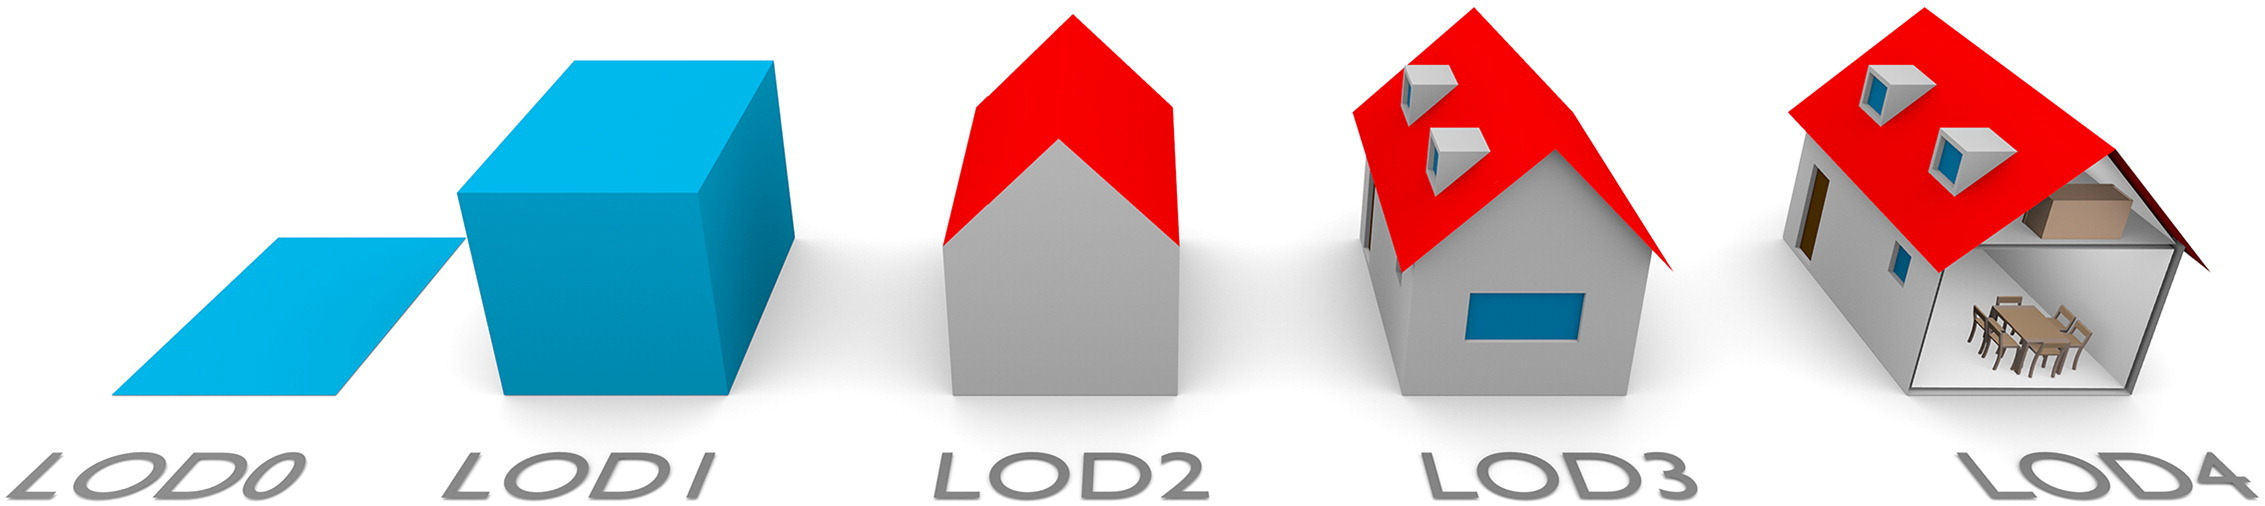
\includegraphics[width=.7\textwidth]{images/introduction/lods}            
                \caption{
                    \label{fig::lods} \gls{acr::lod} categorization used in this work~\parencite{biljecki2016improved}.
                    \gls{acr::lod}-4 is ignored herein.
                }
            \end{figure}
    \subsection{Obstacles in building \gls*{acr::3d} modeling}
        \label{subsec::introduction::urban_3d_reconstruction::challenges}
        The subject of building \gls{acr::3d} modeling has been widely studied in more than twenty years.
        Still, there are some unsolved issues in the field~\parencite{musialski2013survey, lafarge2015some}.
        Presented here is the same classification as in~\textcite{lafarge2015some}.

        \subsubsection{Data acquisition}
            Related to sensor data acquisition are some serious issues, in signal processing in general, just as in \gls{acr::3d} modeling in particular.
            In fact, noise is an integral part of physical measurement processes.
            One should take good care in avoiding error propagation through their processing pipelines.
            For instance, outliers in point-of-interest detection can render a photogrammetrically constructed mesh accumulate sizable geometric errors.\\
            Missing data is also a real issue in \gls{acr::3d}, as some background objects in the scene could be easily occluded by objects in the foreground.
            One way of dealing with this type of obstacles, is to multiply the data acquisition settings.
            This can, actually, help mitigate not only occlusion problems but also noise interference.\\
            However, too much data heterogenuity can also hinder the \gls{acr::3d} modeling process.
            In fact, with more accessible data acquired using different sensors (cameras, \gls{acr::radar} and \gls{acr::lidar}, for instance), in various settings (aerial, sattelite or terrestrial) and circumstances (rainy, sunny, foggy\dots and night-time, day-time\dots), other hurdles need to be overcome.
            For one, more data does not always mean more knowledge, as demonstrated in~\textcite{brachmann2018learning}.
            In fact, one should take good care in choosing how to fuse their input data~\parencite{kedzierski2014terrestrial}.
            For instance, it needs be coregistered in the same referential~\parencite{monnier2013registration, mezian2016uncertainty} (\textit{cf.} Figure~\ref{fig::3d_model_terrestrial_registration}).
            There can also be variabilities in radiometry that needs to be taken into account.\addref
            \begin{figure}[htpb]
                \centering
                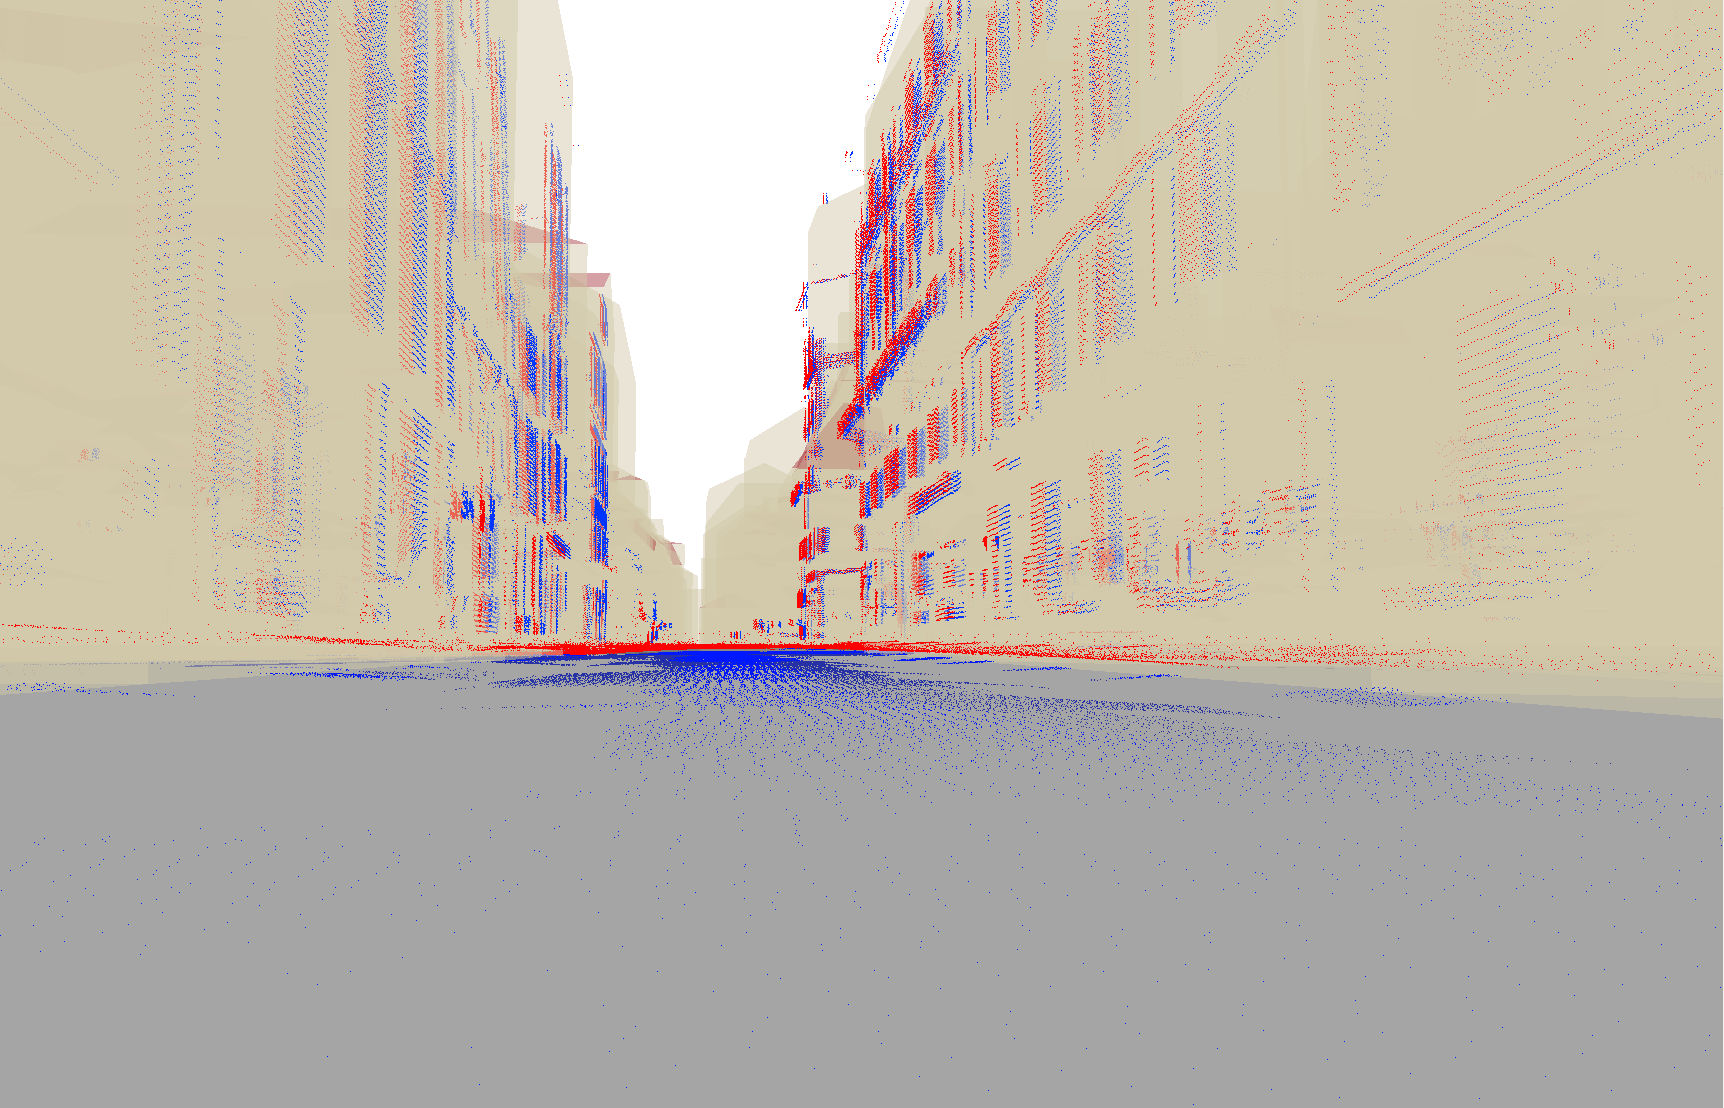
\includegraphics[width=.48\textwidth]{images/introduction/registration_1}
                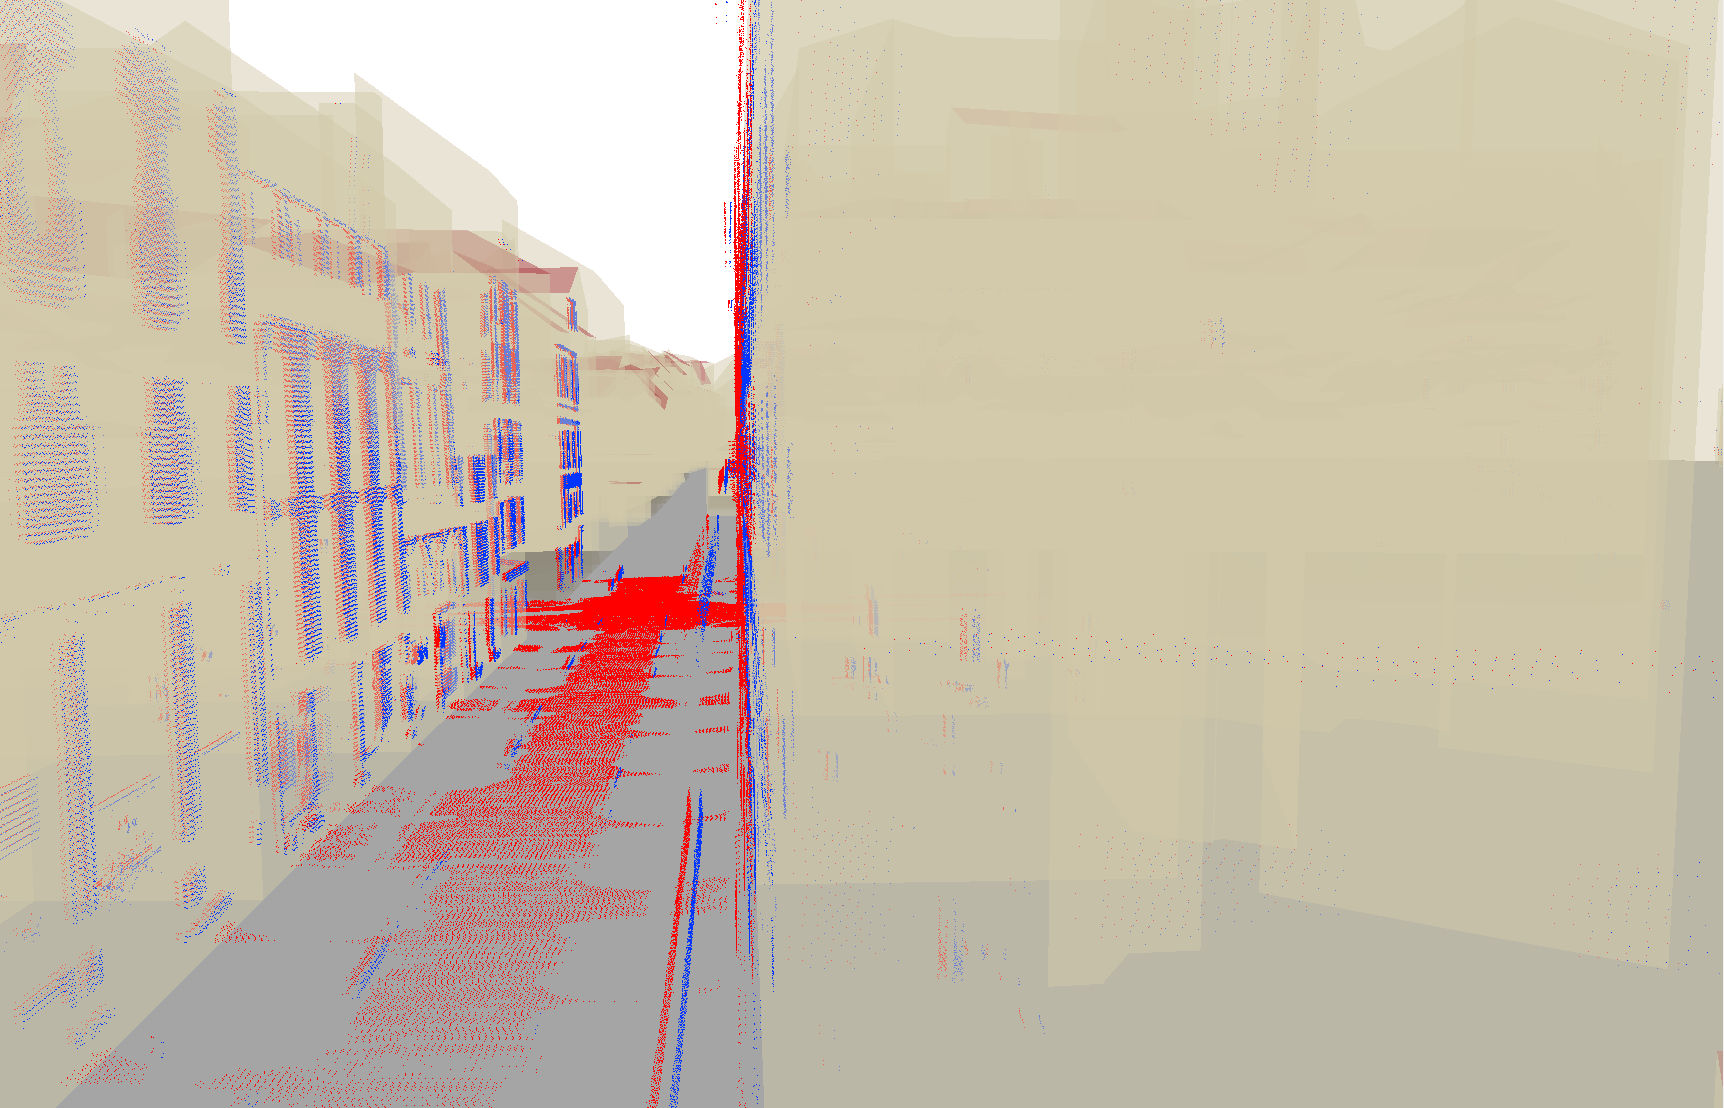
\includegraphics[width=.48\textwidth]{images/introduction/registration_2}
                \caption{
                    \label{fig::3d_model_terrestrial_registration} Terrestrial \gls{acr::lidar} point clouds are registred against building \gls{acr::3d} models~\parencite{monnier2014}.
                    The registred point clouds could be used to enrich the \gls{acr::3d} models with detailed reconstructions of fa\c{c}ades.
                    In \textcolor{Red}{red}, are represented the raw point cloud while the registred one is illustrated in \textcolor{Blue}{blue}.
                }
            \end{figure}

        \subsubsection{Modeling automation}
            The most accurate approach to produce semantically aware and geometrically accurate representations of a building is a manual one.
            It can be either based on high accuracy \textit{in situ} geodetic measurements (errors are of the order of \SI{5}{\cm}~\parencite{kaartinen2005accuracy}).
            Although, it is the most accurate representation possible, it is an arduous and expensive process.
            Stereo-plotting consists on using couples of overlapping images in order to manually determine the \gls{acr::3d} geometry of lines.
            It can be used in building modeling to manually plot building edges in \gls{acr::3d} and hence extract its surface.
            This reduces the complexity of the manual modeling process.
            It produces however lower precision models as errors are of the order of \SI{50}{\cm}~\parencite{jamet1995building}.
            This is still a slow process that is highly demanding in terms of operator expertise~\parencite{ruther2002application}.\\
            The manual labour can be alleviated, partially, by automating some parts of the \gls{acr::3d} surface aquisition pipeline~\parencite{musialski2013survey}.
            Some interactive approaches have been proposed to model building.
            The operator is still needed for highly complex semantic tasks~\parencite{mayunga2005semi, castellazzi2015laser}.
            Such methods suffer from imprecision compared to the fully manual ones: for instance,~\textcite{mayunga2005semi} produces models with geometric error standard deviation in the order of \SI{1}{\m}.\\
            Full automation, although not requiring a lot of ressources, is far from being perfect, especially when it comes to semantics.
            Different strategies are used, where each targets a specific resolution, balancing between compaction and geometric accuracy.
            Ordered from the most to the less compact, these strategies are listed herein.
            In a Manhattan-world setting, one assumes that buildings are collections of boxes~\parencite{vanegas2010building, li2016manhattan}.~\textcite{lafarge_ijcv12, nan2017polyfit}
            relied on the hypothesis that building are made of piecewise planar primitives.
            Rich grammars can give rise to less compact but more accurate models, as is the case of~\textcite{demir2015procedural} or~\textcite{zeng2018neural}.
            Mesh simplification strategies comes last in terms of compaction~\parencite{verdie2015lod, zhou20102}.
            A sketch of this comparison is presented in Figure~\ref{fig::modeling_strategies}.\\
            \begin{figure}[htpb]
                \centering
                \includestandalone[mode=buildnew, width=\textwidth]{figures/modeling_approaches}            
                \caption{
                    \label{fig::modeling_strategies} Modeling strategies and the targeted compaction and geometric accuracy.
                    Depending on the final use of the model, a compromise is chosen between the model compaction and its geometric accuracy.
                }
            \end{figure}
            The compromise, between compaction and geometric precision, relies on an \textit{a prioiri} knowledge of the modeled urban scene.
            Such hypotheses does not naturally hold at large scales.
            Multiple factors play a role in architectural styles of buildings that do not always go hand in hand:
            a geographic proximity does not imply always a temporal or architectural closeness for buildings as depicted in Figure~\ref{subfig::xiiith_paris_haussmann_tower}.
            At a regional or continental scale, the differences become even more overt: \textit{c.f.} Figure~\ref{subfig::different_regions}.
            As a result, some choose to alternate automatic and interactive methods~\parencite{musialski2013survey}: an automatic reconstruction followed by a interactive correction step.
            \begin{figure}[htpb]
                \begin{subfigure}{.48\textwidth}
                    \begin{center}
                        \includegraphics[width=\textwidth]{example-image}
                        \caption{
                            \label{subfig::xiiith_paris_haussmann_tower} Example of two nearly located buildings, in the XIIIth disctict of Paris, with different architectural styles:
                            a Haussmann style building, dating from the begining of the XXth century, next to very tall tower, built \textit{circa} 1970s.
                        }
                    \end{center}
                \end{subfigure}
                \hfill
                \begin{subfigure}{.48\textwidth}
                    \begin{center}
                        \includegraphics[width=\textwidth]{example-image}
                        \caption{
                            \label{subfig::different_regions} Example of two buildings from two different locations in the world:
                            Blalallala.
                        }
                    \end{center}
                \end{subfigure}
                \caption{
                    \label{fig::different_styles} Building architecture shows high heterogenuity not only across different regions, but also in the same urban scene.
                }
            \end{figure}
        
        \subsubsection{Quality evaluation}
            As discussed profusely, semantics play a prominent role in building \gls{acr::3d} models.
            Naturally, it should also be taken into account in the evaluation process.
            It is easier said than done.
            Usually, it is indirectly checked using the compaction criterion~\parencite{lafarge_ijcv12}.\\
            Up to now most studies try to evaluate the quality of modeling algorithms by assessing the accuracy of the geometry of a handfull of buildings.
            These evaluation approaches rely on purely geometric metrics (usually the \gls{acr::rmse}) to compare the reconstructed building to a reference models.
            In a large scale setting, this becomes prohibitive.
            In fact, it means that one should reconstruct, at least, a whole disctict to be able to judge a city model.
            This is expensive in ressources and time.
            Alternatively, many works favor visual inspection of models.
            This requires, in average, \SI[per-mode=repeated-symbol]{2}{\hour\per\km\squared\per\expert}, and in worst case scenarios, as time-consuming  as stereo-plotting the building in the first place.\\
            In the next section, we will discuss, in details, the various ways of evaluating a building model.

\section{Evaluating building models}
    \label{sec::introduction::building_model_evaluation}
    We have just seen how building model quality evaluation is one the main challenges in the field.
    In this section, are presented the different types of quality assessement a building model can undergo.
    First, in subsection~\ref{subsec::introduction::building_model_evaluation::topological}, is described how models could be checked for their topological consistency.
    On the other hand, the \gls{acr::3d} model geometry has also to be checked against the real building geometry.
    This issue is visited in subsection~\ref{subsec::introduction::building_model_evaluation::geometric}.
    Manual geometric inspection is discussed before considering automatic evaluation and its challenges.

    \subsection{Topological consistency inspection}
        \label{subsec::introduction::building_model_evaluation::topological}
        Extensive work has been accomplished, in the past, in order to achieve a standardized representation of city \gls{acr::3d} models.
        This has resulted in the \gls{acr::ogc} CityGML standard\footnote{\href{https://www.opengeospatial.org/standards/citygml}{CityGML}}.
        However, in practice, it is not always respected, as shown in~\textcite{biljecki2016most}, where up to 89\% of models were found to be topologically invalid.\\

        In consequence, the subject of automatic inspection of the topological consistency of city models has drawn a strong attention in the \gls{acr::gis} community.
        The basic common principle is the two-manifoldness of surface representations~\parencite{groger2011achieve}, which aims at excluding self-intersections.
        It is however not sufficient for the complex building cases.
        An urban object, in the international standards is, in reality, represented as an agregation of two-manifold surfaces, as shown in~\textcite{groger2011achieve, ledoux2013validation}.
        This kind of structures can be simply modeled as a \gls{acr::3d} \gls{acr::lcc}\parencite{damiand2014combinatorial}\footnote{
            An nD \gls{acr::lcc} is an embedding of combinatorial maps in \(\mathbb{R}^n\).
        }, as demonstrated in \textcite{diakite2014topological}.
        This leads to the use of \gls{acr::3d} \glspl{acr::lcc} to check the sanity of city models~\parencite{gorszczyk2016automatic}.
        The idea relies, however, on the presence of reference data to compare to.
        While being very useful for format conversion, consistency checks, as intended in the original paper, are pointless when inspecting \gls{acr::3d} models in the wild.\\
        Not all efforts did fully explore the topological possiblities that are provided by the standard~\parencite{biljecki2016most, ledoux2013validation}.
        In fact, most assume that polygons and solids in the representation are not allowed to have holes, like the work of~\textcite{groger2011achieve, alam2014towards}.
        This was, however, the case of~\textcite{ledoux2013validation}.
        Their work built on the axioms of~\textcite{groger2011achieve}: it does not only deal with polygons and surfaces, but also takes care of solids and allows holes of different dimensions (polygons with holes, surfaces with boundaries\footnote{
            This is actually taken into account by the 2.8D models in~\textcite{groger2011achieve}.
        } and volumes with cavity).
        The errors are organized in increasing order of the geometric dimension of the object they affect.
        The process stops at the dimension of the first detected inconsistancies and ignores the higher ones. 
        An open source library and a web-application are publically available~\parencite{ledoux2018val3dity}, in order to further the sanity of exchanged \gls{acr::3d} models of urban scenes.\\

        We should also mention the efforts made to fix the invalid models. 
        These methods could be divided into local and global ones.
        \begin{itemize}
            \item \textbf{Local approaches}: they rely on local topological operators to solve detected issues in the model.
                One such method is CityDoctor~\parencite{alam2014towards}.
                On the downside, these methods have the tendency to introduce more errors in the hope of solving present ones.
                In fact, the problem is often ill-posed, and multiple solutions can be suggested to alleviate the same problem.
            \item \textbf{Global approaches}: the idea is to represent models as volumes constrained by the defectuous surfaces.
            The goal here, as in urban reconstruction, is to infere topological information from the observed geometric properties, taking into account the unreliability of the data as well as \textit{a priori} information on the model.
            This is the case of~\textcite{zhao2013automatic}, which relies on a tetrahydralization of the input model volume and a heuristic carving of unnecessary 3-simplices.
            This approach, in fact, resembles the surface reconstruction procedures from unstructured point clouds using Delaunay triangulation~\parencite{cazals2006delaunay, berger2014state}.
        \end{itemize}

    \subsection{Geometric inspection}
        \label{subsec::introduction::building_model_evaluation::geometric}
        Guarantying topological consistency is a necessary criterion for the quality of city \gls{acr::3d} models.
        It is, however, not sufficient.
        One would want to assess how close is the building geometry to the reality.
        This is what we denote by geometric quality evaluation.\\
        This issue has attracted a lot of attention in \gls{acr::2d}~\parencite{mooney2010towards}, but is not as popular in \gls{acr::3d}.
        This is maybe due to the lesser consideration that is given to the latter.
        This can be explained by the different levels of difficulty when producing these data.
        It is indeed a more difficult to reconstruct a \gls{acr::3d} model of a building than detecting their footprint.
        For example, one can take a look in the number of submission for each task of the proposed \gls{acr::isprs} benchmark~\textcite{rottensteiner2012isprs, rottensteiner2014results}.
        The \gls{acr::3d} reconstruction task received less submissions than the other one.\\
        Two ways can be used to judge the quality of the geometric representation of a building.
        Manual evaluation relies on human interaction to determine how close the model is to reality.
        The automatic approach relies only on the model and other external data to do so without involving a human in the loop.
        Both are discussed herein.

        \subsubsection{Manual evalutation}
            Manual inspection involves a human operator checking the validity of the reconstructed geometry compared to a reference data.
            The lastter could be classified into two types:
            \begin{itemize}
                \item Reference building \gls{acr::3d} models: these are high quality models that were manually produced.
                    One approach is to acquire these on the field by topographic survey.
                    This is, nevertheless, very expensive.
                    Another alternative is to use stereoplotted models using oriented images.
                    This is a more affordable and scalable but a less accurate solution.
                \item Reference sensor data: they are used by operators in constrast with what is examined the geometry of a building model.
                    Oriented images, \gls{acr::dsm} and point clouds are instances of such data.
                    This setting is, with the same or less positional accuracy as the previous case, the easiest to adopt in a large scale.
            \end{itemize}

            Manual inspection is, actually, ideal in the sense that humans are naturally most suited to detect semantic flaws in building representation.
            The latter are, however, not so adapted for quantitative comparisons.
            One way to alleviate such difficulties is to provide software tools to help measuring inaccuracies in geometry\addref.\\

            In contrast, the most persistant issue is scalability.
            Manual inspection is indeed a laborious task that requires some kind of expertise in the field, for a reasonable efficiency.
            Humans are also not so infallible when assigned precise repetitive jobs.
            Human involvement in the reconstruction effort is, actually, one of the reasons behind topological inconsistancies in \gls{acr::3d} models.

        \subsubsection{Automatic evalutation}
            In order to achieve scalability, the get-go solution is automation, failing that a semi-automation.
            As usual, it is easier said than done.\\

            Methods have been proposed to automatically assess building model geometry.
            They rely, however, on ratios that describe the global quality of the model compared to a reference data.
            The flaws are twofold in this case.
            First, global ratios do not capture the finer details in the building.
            Second, reference \gls{acr::3d} models are not cheap to acquire, as discussed earlier.
            While the first issue is a manageable issue, as proven in~\textcite{rottensteiner2012isprs}, the second is not so easy to mitigate.\\

            The most crucial problem is, in constrast, the semantic aspect of the quality assessement.
            As discussed, the models in question possess high semantic properties that have a sizable effect on their geometry.
            Assessing one without the other is fundamentally unsound.
            While this is easy to achieve manually, it has yet to be incorporated in automatic settings.
\section{Contributions}
    \label{sec::introduction::contributions}
    Based on all the previous discussions, we adopted a research direction that was rarely taken up to now, as far as we know.
    Herein is explained the path that led to this subject.
    To do so, the context of this work is explained in detail in subsection~\ref{subsec::introduction::contributions::positioning}.
    Further on, promising and conceivable utilizations are stated in subsection~\ref{subsec::introduction::contributions::use}.
    This is before ending with a summary of the main contributions of this work (\textit{c.f.} subsection~\ref{sec::introduction::contributions::contributions}).
    
    \subsection{Positioning}
        \label{subsec::introduction::contributions::positioning}
        As seen in the previous section (\textit{ie.} section~\ref{sec::introduction::building_model_evaluation}), geometry evaluation of building \gls{acr::3d} models remains a field open for invetigation.
        Topology consistency inspection, in contrast, as discussed in subsection~\ref{subsec::introduction::building_model_evaluation::topological}, has received ample attention from the \gls{acr::gis} community.
        In consequence, it will not be of interest in this work.\\

        Building model evaluation is, herein, studied under two constraints: \textbf{large scale} and \textbf{automation}.
        Each one will have an impact on what settings are to be considered.
        Below, explained are the consequences of each constraint.\\

        Building modeling has been shown, earlier (\textit{cf.} subsection~\ref{subsec::introduction::urban_3d_reconstruction::building_3d_modeling}), to be a bottleneck for urban outdoor modeling at large scales.
        As a consequence, evaluating building \gls{acr::3d} models is essential for entire scene model inspection.
        The difference between buildings and most urban elments is the significance of semantics (\textit{cf.} subsection~\ref{subsec::introduction::urban_3d_reconstruction::building_3d_modeling}).
        The latter translates into structural geometric properties that are not faithfully captured by geometric fidelity metrics.
        As a consequence, the proposed approach should factor semantics in the evaluation.
        As a result, like with \glspl{acr::lod}, errors are exptected to be discretized owing to the semantic character of the evaluation.
        Due to the large scale of the study, the proposed categorization must be stable no matter how the treated urban scene change.\\

        Semantically aware inspection is natural for human operators.
        It is, however, difficult to automate.
        First, models could result from different pipelines and heterogenuous sensors.
        Consequently, the automatic evaluation approach has to be independent from the used building modeling method.
        It has also to take into consideration the \gls{acr::lod} of input models.
        These requirements are not easy to formalize.

    \subsection{Potential use}
        \label{subsec::introduction::contributions::use}
        Ahead was discussed the context of the proposed work.
        Hereafter is discussed the potential use of a semantically aware automatic geometry evaluation of building \gls{acr::3d} models.
        \subsubsection{Change detection}
            This is possible in two ways.
            First, one can consider the same approach that is used for error detection as a method for change detection in building \gls{acr::3d} models.
            This is equivalent to considering change as an semantic error that impacts the geometry of the building.
            Second is the fact that change can be implicitly detected from geometric errors.
            In fact, the change that can be observed from sensor data, will render the outdated model invalid geometrically.
            \begin{figure}[H]
                \centering
                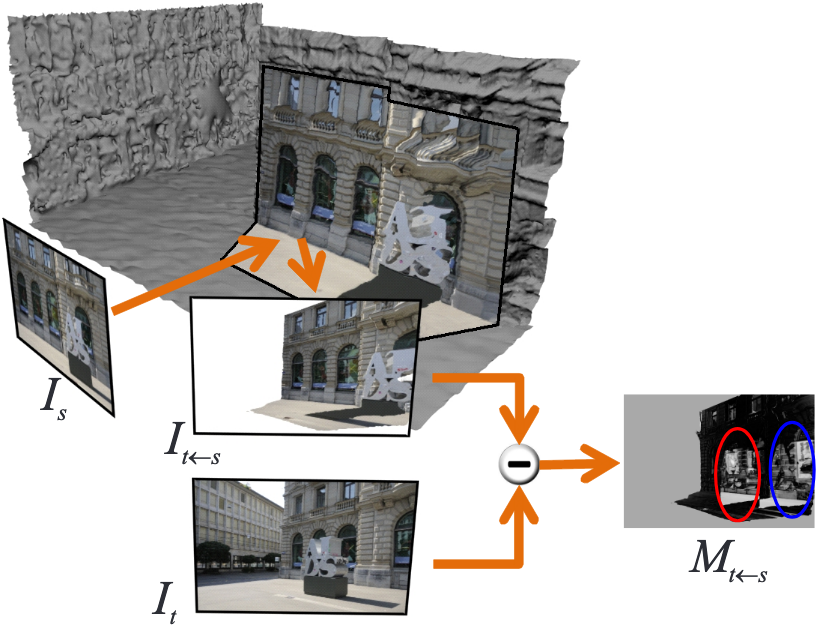
\includegraphics[width=\textwidth]{images/introduction/use/change_detection_taneja}
                \caption{\label{fig::3d_change_detection} Illustration of change detection in urban areas~\parencite{taneja2013city}.}
            \end{figure}

        \subsubsection{Building model correction}
            This is the most obvious usecase for this work.
            In practice, errors are detected by operators in order to correct them.
            The first task, if automated, can be time saving in the correction post-processing step.
            It is even possible to automate the whole correction process using the advances achieved in interactive reconstruction~\parencite{kowdle2011active}.
            \begin{figure}[H]
                \centering
                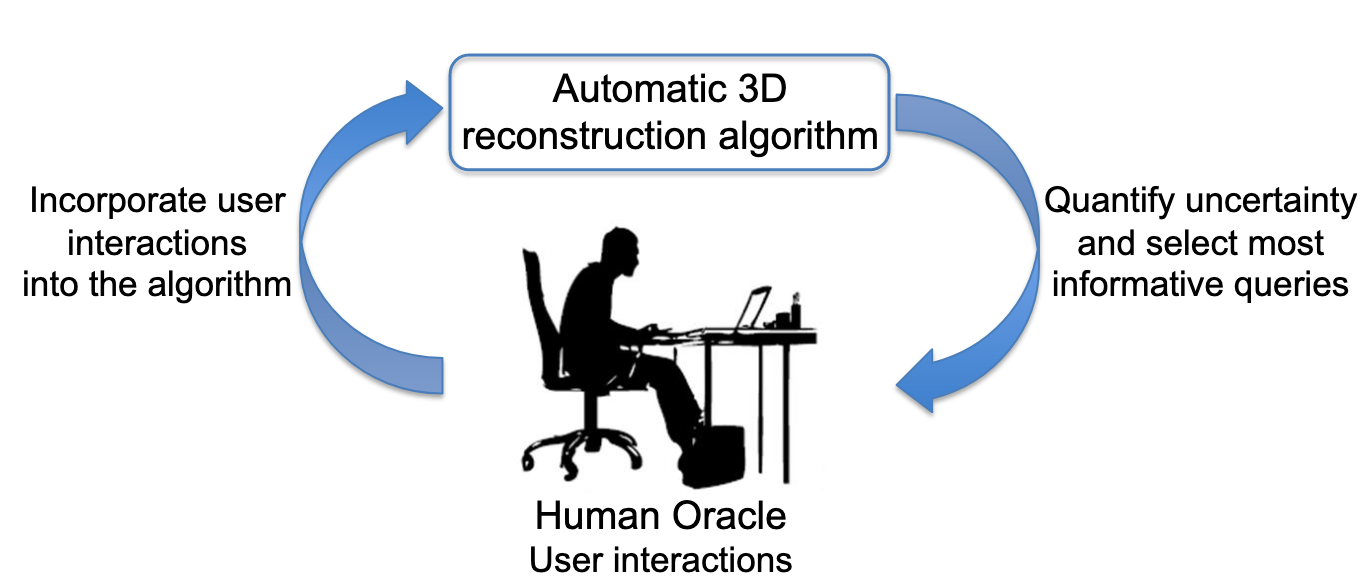
\includegraphics[width=\textwidth]{images/introduction/use/active_learning_kowdle}
                \caption{\label{fig::corrections} Example of an interactive pipeline that needs human operators to provide correct initial reconstructions~\parencite{kowdle2011active}.}
            \end{figure}

        \subsubsection{Reconstruction method selection}
            Evaluation of the building models can help selecting the most adapted reconstruction methods for a certain urban scene.
            Indeed, depending on the needs of the potential final user, some errors are to be watched more than others.
            As an example, an insurance agent, who is only interested in flood simulations, will not be bothered by the geometric accuracy of \gls{acr::lod}-2 features and will focus principally at the \gls{acr::lod}-1 representation errors.
            Modeling algorithms are naturally biased towards a certain setting that depends on the hypotheses chosen by their creators.
            They will produce less errors when those conjectures are met and fail otherwise.
            These assumptions are fixed, for instance, in terms of building types (Haussmann style, Manhattan-world \dots), geometric criterea (planar surfaces, symmetry \dots).
            Hence, choosing a modeling approach can determine how good are the models and vice versa.
            \begin{figure}[H]
                \centering
                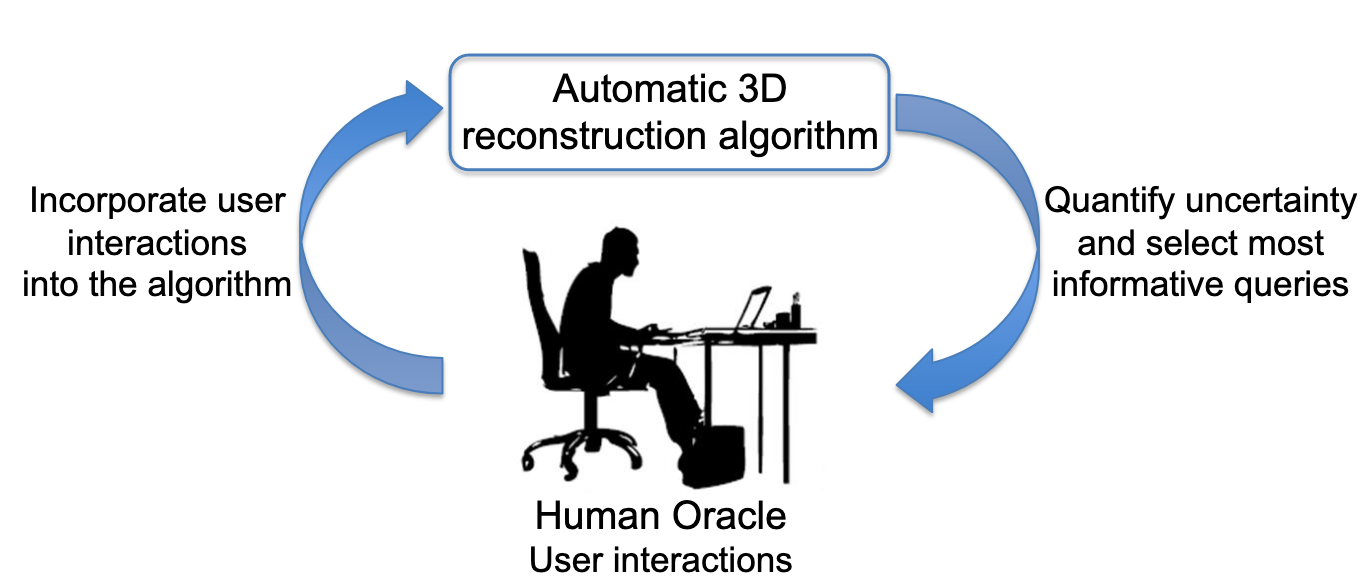
\includegraphics[width=\textwidth]{images/introduction/use/active_learning_kowdle}
                \caption{\label{fig::comparison} Depiction of different models for the same building~\parencite{li2016manhattan}.}
            \end{figure}

            \subsubsection{Crowdsourcing evaluating}
            Crowdsourcing~\parencite{kovashka2016crowdsourcing} can be seen as a building modeling method.
            It has become easier with the help of some online tools like SketchUp\footnote{
                \href{https://www.sketchup.com}{SketchUp}
            }, where anyone can model, for instance, their home and share it publically.
            The quality of the models depend on their author.
            An automatic evaluation method can help check that the uploaded models respect the specifications.
            Another issue is the presence of vandalism in open data~\parencite{neis2012towards}.
            The presented approach can be used to help understandin user behaviors and detect vandaliser.
            \begin{figure}[H]
                \centering
                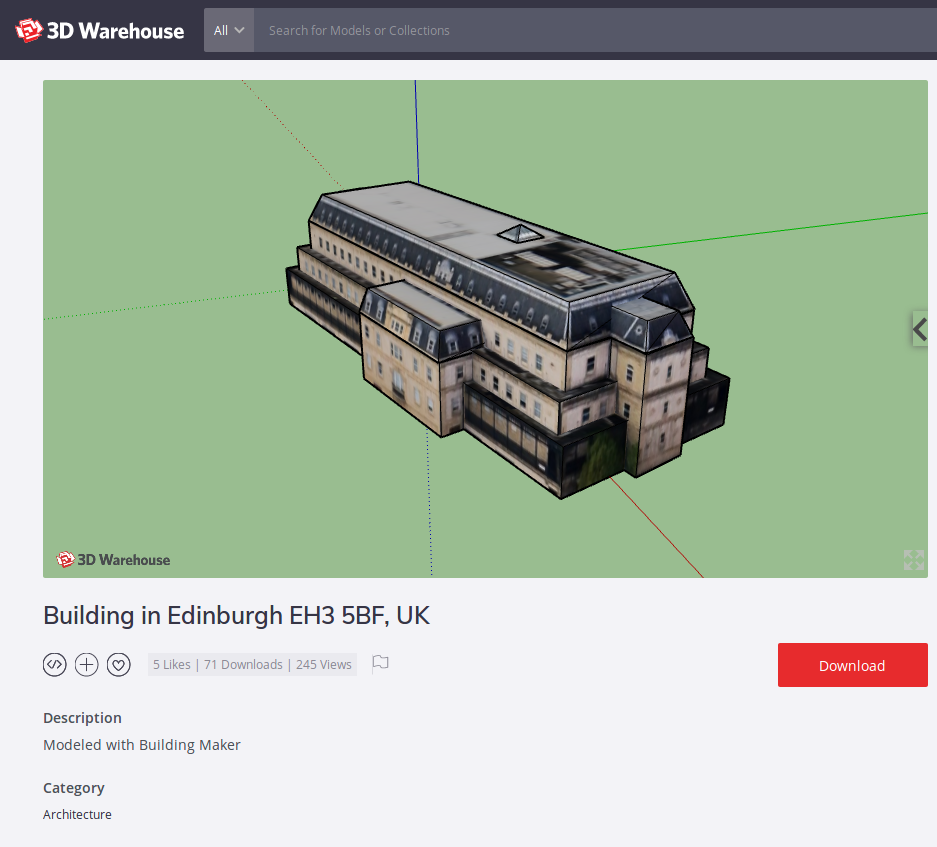
\includegraphics[width=\textwidth]{images/introduction/use/crowdsourcing}
                \caption{\label{fig::crowdsourcing} A sample of a building model made by a SketchUp user.}
            \end{figure}

    \subsection{Main contributions}
        \label{sec::introduction::contributions::contributions}
        Based on the detailed discussion hereinabove, we present our contributions in the field of geometric evaluation of building \gls{acr::3d} models.
        They are three-fold.
        A graphical abstract is presented in Figure~\ref{fig::graphical_abstract} giving an overview of our contributions.
        \begin{figure}[htpb]
            \centering
            \includestandalone[mode=buildnew, width=\textwidth]{figures/graphical_abstract/graphical_abstract}            
            \caption{
                \label{fig::graphical_abstract} Our semantic evaluation framework for 3D building models (a).
                Semantic errors affecting the building are predicted using a supervised classifier and handcrafted features.
                In addition to the input model topological structure (b), features are extracted from Very High resolution overhead data.
                It can be based on a comparison with the \gls*{acr::dsm} (c).
                Optical images can also be used through, for instance, local gradient extraction (d).
                Several errors can be detected at the same time, in a hierarchical manner (e).
                Fidelity errors correspond to geometrical imprecision as shown in red.
                On the other hand, modeling errors denote morphological inconsistancies with the real object.
            }
        \end{figure}
        \subsubsection{Error taxonomy}
            A hierarchical and adaptive taxonomy of errors is proposed.
            It is designed to be independent from the urban scene or the modeling approach.
            In order to achieve this, errors are chosen meticulously as a compromise between generalization and expressivity.
            The first ensures that errors from the taxonomy can fit any scene, while the second implies that errors are not equivocal.
            It is also an adaptive categorization, since, depending on the final user needs, a set of errors can be extracted after specifying some parameters.
            
        \subsubsection{\gls*{acr::3d} model reference free evaluation}
            Acquiring \gls{acr::3d} reference models is very expensive in ressources and particularly not scalable at large scale.
            As a consequence, the problem is formulated as a supervized learning one.
            Based on the errors, that are extracted from the taxonomy, a classifier is trained in order to predict defects for unseen models.

        \subsubsection{Feature baseline}
            Since the formulated problem has not been massively studied, there was no feature extraction baseline to compare to.
            Hence, a baseline of features is presented in this work.
            They are computed based on the geometric attributes of the building model and the comparison to external data: optical images and height maps.
        
        \subsubsection{Scalability}
            One of the goals of this work is to acheive scalability in large scale.
            This implies the transferability of the learned predictors to unseen urban settings or untested modeling techniques.
            It involves also a representativeness and generalization study of the training sets.
            An analysis is conducted accordingly.
            We experimentaly prove the stability of classifiers, under some conditions.

\section{Structure of the Thesis}
    \label{sec::introduction::structure_of_thesis}
